
%%%%%%%%%%%%%%
%% Run LaTeX on this file several times to get Table of Contents,
%% cross-references, and citations.

%% If you have font problems, you may edit the w-bookps.sty file
%% to customize the font names to match those on your system.

%% w-bksamp.tex. Current Version: Feb 16, 2012
%%%%%%%%%%%%%%%%%%%%%%%%%%%%%%%%%%%%%%%%%%%%%%%%%%%%%%%%%%%%%%%%
%
%  Sample file for
%  Wiley Book Style, Design No.: SD 001B, 7x10
%  Wiley Book Style, Design No.: SD 004B, 6x9
%
%
%  Prepared by Amy Hendrickson, TeXnology Inc.
%  http://www.texnology.com
%%%%%%%%%%%%%%%%%%%%%%%%%%%%%%%%%%%%%%%%%%%%%%%%%%%%%%%%%%%%%%%%

%%%%%%%%%%%%%
% 7x10
%\documentclass{wileySev}

% 6x9
\documentclass{wileySix}

\usepackage{graphicx}
\usepackage{listings}
\usepackage{float}
\usepackage{color}

\definecolor{codegreen}{rgb}{0,0.6,0}
\definecolor{codegray}{rgb}{0.5,0.5,0.5}
\definecolor{codepurple}{rgb}{0.58,0,0.82}
\definecolor{backcolour}{rgb}{0.95,0.95,0.92}

\lstdefinestyle{mystyle}{
    backgroundcolor=\color{backcolour},
    commentstyle=\color{codegreen},
    keywordstyle=\color{magenta},
    numberstyle=\tiny\color{codegray},
    stringstyle=\color{codepurple},
    basicstyle=\footnotesize,
    breakatwhitespace=false,
    breaklines=true,
    captionpos=b,
    keepspaces=true,
    numbers=left,
    numbersep=5pt,
    showspaces=false,
    showstringspaces=false,
    showtabs=false,
    tabsize=2,
    language=sh
}

\lstset{style=mystyle}

%%%%%%%
%% for times math: However, this package disables bold math (!)
%% \mathbf{x} will still work, but you will not have bold math
%% in section heads or chapter titles. If you don't use math
%% in those environments, mathptmx might be a good choice.

% \usepackage{mathptmx}

% For PostScript text
\usepackage{w-bookps}

%%%%%%%%%%%%%%%%%%%%%%%%%%%%%%%%%%%%%%%%%%%%%%%%%%%%%%%%%%%%%%%%
%% Other packages you might want to use:

% for chapter bibliography made with BibTeX
% \usepackage{chapterbib}

% for multiple indices
% \usepackage{multind}

% for answers to problems
% \usepackage{answers}

%%%%%%%%%%%%%%%%%%%%%%%%%%%%%%
%% Change options here if you want:
%%
%% How many levels of section head would you like numbered?
%% 0= no section numbers, 1= section, 2= subsection, 3= subsubsection
%%==>>
\setcounter{secnumdepth}{3}

%% How many levels of section head would you like to appear in the
%% Table of Contents?
%% 0= chapter titles, 1= section titles, 2= subsection titles,
%% 3= subsubsection titles.
%%==>>
\setcounter{tocdepth}{2}

%% Cropmarks? good for final page makeup
%% \docropmarks

%%%%%%%%%%%%%%%%%%%%%%%%%%%%%%
%
% DRAFT
%
% Uncomment to get double spacing between lines, current date and time
% printed at bottom of page.
% \draft
% (If you want to keep tables from becoming double spaced also uncomment
% this):
% \renewcommand{\arraystretch}{0.6}
%%%%%%%%%%%%%%%%%%%%%%%%%%%%%%

%%%%%%% Demo of section head containing sample macro:
%% To get a macro to expand correctly in a section head, with upper and
%% lower case math, put the definition and set the box
%% before \begin{document}, so that when it appears in the
%% table of contents it will also work:

\newcommand{\VT}[1]{\ensuremath{{V_{T#1}}}}

%% use a box to expand the macro before we put it into the section head:

\newbox\sectsavebox
\setbox\sectsavebox=\hbox{\boldmath\VT{xyz}}

%%%%%%%%%%%%%%%%% End Demo


\begin{document}


\booktitle{Cerdas Menguasai Python}
\subtitle{Dalam 24 Jam}

\authors{Rolly M. Awangga\\
\affil{Informatics Research Center}
%Floyd J. Fowler, Jr.\\
%\affil{University of New Mexico}
}

\offprintinfo{Cerdas Menguasai Python, First Edition}{Rolly M. Awangga}

%% Can use \\ if title, and edition are too wide, ie,
%% \offprintinfo{Survey Methodology,\\ Second Edition}{Robert M. Groves}

%%%%%%%%%%%%%%%%%%%%%%%%%%%%%%
%%
\halftitlepage

%\titlepage


\begin{copyrightpage}{2019}
%Survey Methodology / Robert M. Groves . . . [et al.].
%\       p. cm.---(Wiley series in survey methodology)
%\    ``Wiley-Interscience."
%\    Includes bibliographical references and index.
%\    ISBN 0-471-48348-6 (pbk.)
%\    1. Surveys---Methodology.  2. Social 
%\  sciences---Research---Statistical methods.  I. Groves, Robert M.  II. %
%Series.\\
%
%HA31.2.S873 2007
%001.4'33---dc22                                             2004044064
\end{copyrightpage}

\dedication{`Jika Kamu tidak dapat menahan lelahnya belajar,
Maka kamu harus sanggup menahan perihnya Kebodohan.'
~Imam Syafi'i~}

\begin{contributors}
\name{Rolly Maulana Awangga,} Informatics Research Center., Politeknik Pos Indonesia, Bandung,
Indonesia



\end{contributors}

\contentsinbrief
\tableofcontents
\listoffigures
\listoftables
\lstlistoflistings


\begin{foreword}
Sepatah kata dari Kaprodi, Kabag Kemahasiswaan dan Mahasiswa
\end{foreword}

\begin{preface}
Buku ini diciptakan bagi yang awam dengan flask sekalipun.

\prefaceauthor{R. M. Awangga}
\where{Bandung, Jawa Barat\\
Februari, 2019}
\end{preface}


\begin{acknowledgments}
Terima kasih atas semua masukan dari para mahasiswa agar bisa membuat buku ini 
lebih baik dan lebih mudah dimengerti.

Terima kasih ini juga ditujukan khusus untuk team IRC yang 
telah fokus untuk belajar dan memahami bagaimana buku ini mendampingi proses 
Intership.
\authorinitials{R. M. A.}
\end{acknowledgments}

\begin{acronyms}
\acro{ACGIH}{American Conference of Governmental Industrial Hygienists}
\acro{AEC}{Atomic Energy Commission}
\acro{OSHA}{Occupational Health and Safety Commission}
\acro{SAMA}{Scientific Apparatus Makers Association}
\end{acronyms}

\begin{glossary}
\term{git}Merupakan manajemen sumber kode yang dibuat oleh linus torvald.

\term{bash}Merupakan bahasa sistem operasi berbasiskan *NIX.

\term{linux}Sistem operasi berbasis sumber kode terbuka yang dibuat oleh Linus Torvald
\end{glossary}

\begin{symbols}
\term{A}Amplitude

\term{\hbox{\&}}Propositional logic symbol 

\term{a}Filter Coefficient

\bigskip

\term{\mathcal{B}}Number of Beats
\end{symbols}

\begin{introduction}

%% optional, but if you want to list author:

\introauthor{Rolly Maulana Awangga, S.T., M.T.}
{Informatics Research Center\\
Bandung, Jawa Barat, Indonesia}

Pada era disruptif  \index{disruptif}\index{disruptif!modern} 
saat ini. git merupakan sebuah kebutuhan dalam sebuah organisasi pengembangan perangkat lunak.
Buku ini diharapkan bisa menjadi penghantar para programmer, analis, IT Operation dan Project Manajer.
Dalam melakukan implementasi git pada diri dan organisasinya.

Rumusnya cuman sebagai contoh aja biar keren\cite{awangga2018sampeu}.

\begin{equation}
ABC {\cal DEF} \alpha\beta\Gamma\Delta\sum^{abc}_{def}
\end{equation}

\end{introduction}

%%%%%%%%%%%%%%%%%%Isi Buku_
%TEORI
%\chapter{Judul Bagian Pertama}
%\section{Arjun Yuda Firwanda}
\subsection{Soal 1}
Isi jawaban soal ke-1

Kalau mau dibikin paragrap \textbf{cukup enter aja}, tidak usah pakai \verb|par| dsb

%\subsection{Soal 2}
%Isi jawaban soal ke-2

%\subsection{Soal 3}
%Isi jawaban soal ke-3

\section{Dwi Yulianingsih}
\subsection{Soal 1}
Isi jawaban soal ke-1

Kalau mau dibikin paragrap \textbf{cukup enter aja}, tidak usah pakai \verb|par| dsb

%\subsection{Soal 2}
%Isi jawaban soal ke-2

%\subsection{Soal 3}
%Isi jawaban soal ke-3

\section{Harun Ar-Rasyid}
\subsection{Soal 1}
Isi jawaban soal ke-1

Kalau mau dibikin paragrap \textbf{cukup enter aja}, tidak usah pakai \verb|par| dsb

%\subsection{Soal 2}
%Isi jawaban soal ke-2

%\subsection{Soal 3}
%Isi jawaban soal ke-3

\section{Sri Rahayu}
\subsection{Soal 1}
Isi jawaban soal ke-1

Kalau mau dibikin paragrap \textbf{cukup enter aja}, tidak usah pakai \verb|par| dsb

%\subsection{Soal 2}
%Isi jawaban soal ke-2

%\subsection{Soal 3}
%Isi jawaban soal ke-3

\section{Doli Jonviter}
\subsection{Soal 1}
Isi jawaban soal ke-1

Kalau mau dibikin paragrap \textbf{cukup enter aja}, tidak usah pakai \verb|par| dsb

%\subsection{Soal 2}
%Isi jawaban soal ke-2

%\subsection{Soal 3}
%Isi jawaban soal ke-3

\section{Rahmatul Ridha}
\subsection{Soal 1}
Isi jawaban soal ke-1

Kalau mau dibikin paragrap \textbf{cukup enter aja}, tidak usah pakai \verb|par| dsb

%\subsection{Soal 2}
%Isi jawaban soal ke-2

%\subsection{Soal 3}
%Isi jawaban soal ke-3

\section{Tomy Prawoto}
\subsection{Soal 1}
Isi jawaban soal ke-1

Kalau mau dibikin paragrap \textbf{cukup enter aja}, tidak usah pakai \verb|par| dsb

%\subsection{Soal 2}
%Isi jawaban soal ke-2

%\subsection{Soal 3}
%Isi jawaban soal ke-3

%PRAKTEK
%\chapter{Judul Bagian Pertama}
%\section{Arjun Yuda Firwanda}
\subsection{Soal 1}
Isi jawaban soal ke-1

Kalau mau dibikin paragrap \textbf{cukup enter aja}, tidak usah pakai \verb|par| dsb

%\subsection{Soal 2}
%Isi jawaban soal ke-2

%\subsection{Soal 3}
%Isi jawaban soal ke-3

\section{Dwi Yulianingsih}
\subsection{Soal 1}
Isi jawaban soal ke-1

Kalau mau dibikin paragrap \textbf{cukup enter aja}, tidak usah pakai \verb|par| dsb

%\subsection{Soal 2}
%Isi jawaban soal ke-2

%\subsection{Soal 3}
%Isi jawaban soal ke-3

\section{Harun Ar-Rasyid}
\subsection{Soal 1}
Isi jawaban soal ke-1

Kalau mau dibikin paragrap \textbf{cukup enter aja}, tidak usah pakai \verb|par| dsb

%\subsection{Soal 2}
%Isi jawaban soal ke-2

%\subsection{Soal 3}
%Isi jawaban soal ke-3

\section{Sri Rahayu}
\subsection{Soal 1}
Isi jawaban soal ke-1

Kalau mau dibikin paragrap \textbf{cukup enter aja}, tidak usah pakai \verb|par| dsb

%\subsection{Soal 2}
%Isi jawaban soal ke-2

%\subsection{Soal 3}
%Isi jawaban soal ke-3

\section{Doli Jonviter}
\subsection{Soal 1}
Isi jawaban soal ke-1

Kalau mau dibikin paragrap \textbf{cukup enter aja}, tidak usah pakai \verb|par| dsb

%\subsection{Soal 2}
%Isi jawaban soal ke-2

%\subsection{Soal 3}
%Isi jawaban soal ke-3

\section{Rahmatul Ridha}
\subsection{Soal 1}
Isi jawaban soal ke-1

Kalau mau dibikin paragrap \textbf{cukup enter aja}, tidak usah pakai \verb|par| dsb

%\subsection{Soal 2}
%Isi jawaban soal ke-2

%\subsection{Soal 3}
%Isi jawaban soal ke-3

\section{Tomy Prawoto}
\subsection{Soal 1}
Isi jawaban soal ke-1

Kalau mau dibikin paragrap \textbf{cukup enter aja}, tidak usah pakai \verb|par| dsb

%\subsection{Soal 2}
%Isi jawaban soal ke-2

%\subsection{Soal 3}
%Isi jawaban soal ke-3


%TEORI
%\chapter{Judul Bagian Pertama}
%\section{Arjun Yuda Firwanda}
\subsection{Soal 1}
Isi jawaban soal ke-1

Kalau mau dibikin paragrap \textbf{cukup enter aja}, tidak usah pakai \verb|par| dsb

%\subsection{Soal 2}
%Isi jawaban soal ke-2

%\subsection{Soal 3}
%Isi jawaban soal ke-3

\section{Dwi Yulianingsih}
\subsection{Soal 1}
Isi jawaban soal ke-1

Kalau mau dibikin paragrap \textbf{cukup enter aja}, tidak usah pakai \verb|par| dsb

%\subsection{Soal 2}
%Isi jawaban soal ke-2

%\subsection{Soal 3}
%Isi jawaban soal ke-3

\section{Harun Ar-Rasyid}
\subsection{Soal 1}
Isi jawaban soal ke-1

Kalau mau dibikin paragrap \textbf{cukup enter aja}, tidak usah pakai \verb|par| dsb

%\subsection{Soal 2}
%Isi jawaban soal ke-2

%\subsection{Soal 3}
%Isi jawaban soal ke-3

\section{Sri Rahayu}
\subsection{Soal 1}
Isi jawaban soal ke-1

Kalau mau dibikin paragrap \textbf{cukup enter aja}, tidak usah pakai \verb|par| dsb

%\subsection{Soal 2}
%Isi jawaban soal ke-2

%\subsection{Soal 3}
%Isi jawaban soal ke-3

\section{Doli Jonviter}
\subsection{Soal 1}
Isi jawaban soal ke-1

Kalau mau dibikin paragrap \textbf{cukup enter aja}, tidak usah pakai \verb|par| dsb

%\subsection{Soal 2}
%Isi jawaban soal ke-2

%\subsection{Soal 3}
%Isi jawaban soal ke-3

\section{Rahmatul Ridha}
\subsection{Soal 1}
Isi jawaban soal ke-1

Kalau mau dibikin paragrap \textbf{cukup enter aja}, tidak usah pakai \verb|par| dsb

%\subsection{Soal 2}
%Isi jawaban soal ke-2

%\subsection{Soal 3}
%Isi jawaban soal ke-3

\section{Tomy Prawoto}
\subsection{Soal 1}
Isi jawaban soal ke-1

Kalau mau dibikin paragrap \textbf{cukup enter aja}, tidak usah pakai \verb|par| dsb

%\subsection{Soal 2}
%Isi jawaban soal ke-2

%\subsection{Soal 3}
%Isi jawaban soal ke-3

%PRAKTEK
%\chapter{Judul Bagian Pertama}
%\section{Arjun Yuda Firwanda}
\subsection{Soal 1}
Isi jawaban soal ke-1

Kalau mau dibikin paragrap \textbf{cukup enter aja}, tidak usah pakai \verb|par| dsb

%\subsection{Soal 2}
%Isi jawaban soal ke-2

%\subsection{Soal 3}
%Isi jawaban soal ke-3

\section{Dwi Yulianingsih}
\subsection{Soal 1}
Isi jawaban soal ke-1

Kalau mau dibikin paragrap \textbf{cukup enter aja}, tidak usah pakai \verb|par| dsb

%\subsection{Soal 2}
%Isi jawaban soal ke-2

%\subsection{Soal 3}
%Isi jawaban soal ke-3

\section{Harun Ar-Rasyid}
\subsection{Soal 1}
Isi jawaban soal ke-1

Kalau mau dibikin paragrap \textbf{cukup enter aja}, tidak usah pakai \verb|par| dsb

%\subsection{Soal 2}
%Isi jawaban soal ke-2

%\subsection{Soal 3}
%Isi jawaban soal ke-3

\section{Sri Rahayu}
\subsection{Soal 1}
Isi jawaban soal ke-1

Kalau mau dibikin paragrap \textbf{cukup enter aja}, tidak usah pakai \verb|par| dsb

%\subsection{Soal 2}
%Isi jawaban soal ke-2

%\subsection{Soal 3}
%Isi jawaban soal ke-3

\section{Doli Jonviter}
\subsection{Soal 1}
Isi jawaban soal ke-1

Kalau mau dibikin paragrap \textbf{cukup enter aja}, tidak usah pakai \verb|par| dsb

%\subsection{Soal 2}
%Isi jawaban soal ke-2

%\subsection{Soal 3}
%Isi jawaban soal ke-3

\section{Rahmatul Ridha}
\subsection{Soal 1}
Isi jawaban soal ke-1

Kalau mau dibikin paragrap \textbf{cukup enter aja}, tidak usah pakai \verb|par| dsb

%\subsection{Soal 2}
%Isi jawaban soal ke-2

%\subsection{Soal 3}
%Isi jawaban soal ke-3

\section{Tomy Prawoto}
\subsection{Soal 1}
Isi jawaban soal ke-1

Kalau mau dibikin paragrap \textbf{cukup enter aja}, tidak usah pakai \verb|par| dsb

%\subsection{Soal 2}
%Isi jawaban soal ke-2

%\subsection{Soal 3}
%Isi jawaban soal ke-3


%TEORI
%\chapter{Judul Bagian Pertama}
%\section{Arjun Yuda Firwanda}
\subsection{Soal 1}
Isi jawaban soal ke-1

Kalau mau dibikin paragrap \textbf{cukup enter aja}, tidak usah pakai \verb|par| dsb

%\subsection{Soal 2}
%Isi jawaban soal ke-2

%\subsection{Soal 3}
%Isi jawaban soal ke-3

\section{Dwi Yulianingsih}
\subsection{Soal 1}
Isi jawaban soal ke-1

Kalau mau dibikin paragrap \textbf{cukup enter aja}, tidak usah pakai \verb|par| dsb

%\subsection{Soal 2}
%Isi jawaban soal ke-2

%\subsection{Soal 3}
%Isi jawaban soal ke-3

\section{Harun Ar-Rasyid}
\subsection{Soal 1}
Isi jawaban soal ke-1

Kalau mau dibikin paragrap \textbf{cukup enter aja}, tidak usah pakai \verb|par| dsb

%\subsection{Soal 2}
%Isi jawaban soal ke-2

%\subsection{Soal 3}
%Isi jawaban soal ke-3

\section{Sri Rahayu}
\subsection{Soal 1}
Isi jawaban soal ke-1

Kalau mau dibikin paragrap \textbf{cukup enter aja}, tidak usah pakai \verb|par| dsb

%\subsection{Soal 2}
%Isi jawaban soal ke-2

%\subsection{Soal 3}
%Isi jawaban soal ke-3

\section{Doli Jonviter}
\subsection{Soal 1}
Isi jawaban soal ke-1

Kalau mau dibikin paragrap \textbf{cukup enter aja}, tidak usah pakai \verb|par| dsb

%\subsection{Soal 2}
%Isi jawaban soal ke-2

%\subsection{Soal 3}
%Isi jawaban soal ke-3

\section{Rahmatul Ridha}
\subsection{Soal 1}
Isi jawaban soal ke-1

Kalau mau dibikin paragrap \textbf{cukup enter aja}, tidak usah pakai \verb|par| dsb

%\subsection{Soal 2}
%Isi jawaban soal ke-2

%\subsection{Soal 3}
%Isi jawaban soal ke-3

\section{Tomy Prawoto}
\subsection{Soal 1}
Isi jawaban soal ke-1

Kalau mau dibikin paragrap \textbf{cukup enter aja}, tidak usah pakai \verb|par| dsb

%\subsection{Soal 2}
%Isi jawaban soal ke-2

%\subsection{Soal 3}
%Isi jawaban soal ke-3

%PRAKTEK
%\chapter{Judul Bagian Pertama}
%\section{Arjun Yuda Firwanda}
\subsection{Soal 1}
Isi jawaban soal ke-1

Kalau mau dibikin paragrap \textbf{cukup enter aja}, tidak usah pakai \verb|par| dsb

%\subsection{Soal 2}
%Isi jawaban soal ke-2

%\subsection{Soal 3}
%Isi jawaban soal ke-3

\section{Dwi Yulianingsih}
\subsection{Soal 1}
Isi jawaban soal ke-1

Kalau mau dibikin paragrap \textbf{cukup enter aja}, tidak usah pakai \verb|par| dsb

%\subsection{Soal 2}
%Isi jawaban soal ke-2

%\subsection{Soal 3}
%Isi jawaban soal ke-3

\section{Harun Ar-Rasyid}
\subsection{Soal 1}
Isi jawaban soal ke-1

Kalau mau dibikin paragrap \textbf{cukup enter aja}, tidak usah pakai \verb|par| dsb

%\subsection{Soal 2}
%Isi jawaban soal ke-2

%\subsection{Soal 3}
%Isi jawaban soal ke-3

\section{Sri Rahayu}
\subsection{Soal 1}
Isi jawaban soal ke-1

Kalau mau dibikin paragrap \textbf{cukup enter aja}, tidak usah pakai \verb|par| dsb

%\subsection{Soal 2}
%Isi jawaban soal ke-2

%\subsection{Soal 3}
%Isi jawaban soal ke-3

\section{Doli Jonviter}
\subsection{Soal 1}
Isi jawaban soal ke-1

Kalau mau dibikin paragrap \textbf{cukup enter aja}, tidak usah pakai \verb|par| dsb

%\subsection{Soal 2}
%Isi jawaban soal ke-2

%\subsection{Soal 3}
%Isi jawaban soal ke-3

\section{Rahmatul Ridha}
\subsection{Soal 1}
Isi jawaban soal ke-1

Kalau mau dibikin paragrap \textbf{cukup enter aja}, tidak usah pakai \verb|par| dsb

%\subsection{Soal 2}
%Isi jawaban soal ke-2

%\subsection{Soal 3}
%Isi jawaban soal ke-3

\section{Tomy Prawoto}
\subsection{Soal 1}
Isi jawaban soal ke-1

Kalau mau dibikin paragrap \textbf{cukup enter aja}, tidak usah pakai \verb|par| dsb

%\subsection{Soal 2}
%Isi jawaban soal ke-2

%\subsection{Soal 3}
%Isi jawaban soal ke-3


%TEORI
%\chapter{Library CSV dan Pandas}
%\section{Dini Permata Putri | 1174053}
\subsection{Teori}
\begin{enumerate}

\item Apa itu fungsi file csv, jelaskan sejarah dan contoh\\
jawab : file CSV atau Comma Separated Value seperti namanya berisi teks data yang tiap datanya dipisahkan dengan tanda koma. Sebagai gambaran, sebuah file CSV bisa berisi data berikut ini :\\
HeaderA, HeaderB, HeaderC\\
RowA1, RowB1, RowC1\\
RowA2, RowB2, RowC2\\
Jika kita membuat sebuah file di Excel dan menyimpannya dalam format CSV, maka file tersebut dibuka di Notepad maka akan terlihat isi file yang kurang lebih formatnya sama seperti di atas.\\

\item Aplikasi-aplikasi apa saja yang bisa menciptakan file csv?\\
jawab : microsoft office, dll.\\

\item Jelaskan bagaimana cara menulis dan membaca file csv di excel atau spreadsheet\\
jawab : 1. Buka MS Excel Anda\\
2. Klik Data > Get External Data > From Text\\ 
3. Akan muncul Text Import Wizard, arahkan pada file csv yang ingin anda buka > Open.\\
4. Setelah File terbuka, akan muncul Text Import Wizard\\
Step 1 –> Pilih Delimited, Kemudian Next (Di sini, bisa juga menentukan baris awal yang akan di import)\\
Step 2 –> Centrang pada Tab dan Comma (Atau sesuai pengaturan File Anda) > Next\\
Step 3 –> Atur Format data pada tiap kolom yang tampil dan klik Finish\\

\item Jelaskan sejarah library csv\\
jawab : Jaringan perpustakaan digital pertama di Indonesia mulai beroperasi pada bulan Juni 2001.  Jaringan Perpustakaan Digital tersebut itu bernama IndonesiaDLN (Digital Library Network).  IndonesiaDLN diprakarsai oleh Knowledge Management Research Group (KMRG) Institut Teknologi Bandung (ITB) yang merintis pembuatan jaringan perpustakaan digital (digital library network) antar lembaga pendidikan tinggi.  Jaringan pustaka digital bertujuan mempermudah kalangan akademik dan masyarakat umum untuk mengakses hasil penelitian, tugas akhir mahasiswa, tesis maupun disertasi. Dana awal pengembangan jaringan berasal dari Singapura sebanyak 60.000 dolar Kanada, dan dari Yayasan Litbang Telekomunikasi dan Teknologi Informasi (YLTI) sebanyak Rp 150 juta. \\

Pada awal berdirinya, lembaga yang bergabung dalam jaringan pustaka digital IndonesiaDLN antara lain Proyek Pengembangan Universitas Indonesia Timur, LIPI Jakarta, Universitas Brawijaya Malang, Universitas Muhammadiyah Malang, Lembaga Penelitian ITB, Pasca Sarjana ITB, serta Computer Network Research Group (CNRG).\\

Ketua KMRG saat itu sekaligus sebagai penggagas IndonesiaDLN Ismail Fahmi menjelaskan bahwa ide dasar pengembangan pustaka digital bahwa hasil pemikiran dan penelitian harus bisa dipertukarkan (share) dan diakses secara cepat dan mudah. Copyright untuk tugas akhir maupun penelitian pada dasarnya termasuk public domain kecuali yang terikat pada perjanjian dengan industri atau dalam persiapan untuk mendapatkan hak paten. IndonesiaDLN bertujuan agar hasil-hasil penelitian dari perguruan tinggi maupun lembaga penelitian bisa diakes dari manapun di seluruh penjuru dunia dapat diakses secara mudah dan murah dalam bentuk digital, tanpa memerlukan biaya transportasi maupun fotokopi yang biasanya harus dengan mengeluarkan biaya cukup tinggi.\\

Gagasan pembentukan jaringan perpustakaan nasional ini bermula dari peluncuran situs Ganesha Digital Library/GDL (perpustakaan digital milik ITB) Oktober 2000. Sekitar 20 institusi kemudian terlibat dalam proyek jaringan perpustakaan ini. Beberapa server individu juga ikut menyebarkan informasinya melalui GDL, seperti Onno W. Purbo, Budi Rahardjo, dan Ismail Fahmi.\\

Jaringan pustaka digital ini merupakan satu dari beberapa produk KMRG. Produk lainnya adalah Ganesha digital library, software untuk otomatisasi perpustakaan (GNU-Lib) serta software untuk katalog database perpustakaan\\
(http://isisnetwork.lib.itb.ac.id).\\

Menurut Sekjen IndonesiaDLN,  Ismail Fahmi, jaringan perpustakaan digital ini berfungsi sebagai terminal dari berbagai server di Indonesia yang menyediakan informasi ilmu pengetahuan. Misi jaringan ini adalah mengelola ilmu pengetahuan yang dimiliki bangsa Indonesia, dalam satu jaringan yang terdistribusi dan terbuka.\\

\item Jelaskan sejarah library pandas\\
jawab : engembang Wes McKinney mulai mengerjakan pandas pada 2008 ketika di AQR Capital Management karena kebutuhan akan alat kinerja tinggi yang fleksibel untuk melakukan analisis kuantitatif pada data keuangan. Sebelum meninggalkan AQR, dia bisa meyakinkan manajemen untuk mengizinkannya membuka sumber perpustakaan.\\

Pegawai AQR lainnya, Chang She, bergabung dengan upaya ini pada 2012 sebagai kontributor utama kedua ke perpustakaan.\\

Pada 2015, panda ditandatangani sebagai proyek NumFOCUS yang disponsori secara fiskal, sebuah badan amal nirlaba 501 (c) (3) di Amerika Serikat.\\

\item Jelaskan fungsi-fungsi yang terdapat di library csv\\
jawab : Jika kita membuat sebuah file di Excel dan menyimpannya dalam format CSV, maka file tersebut dibuka di Notepad maka akan terlihat isi file yang kurang lebih formatnya sama seperti di atas.\\

\item Jelaskan fungsi-fungsi yang terdapat di library pandas\\
jawab : dapat mengolah suatu data dan mengolahnya seperti join, distinct, group by, agregasi, dan teknik seperti pada SQL. Hanya saja dilakukan pada tabel yang dimuat dari file ke RAM.\\

Pandas juga dapat membaca file dari berbagai format seperti .txt, .csv, .tsv, dan lainnya. Anggap saja Pandas adalah spreadsheet namun tidak memiliki GUI dan punya fitur seperti SQL.\\
\end{enumerate}

%%%%%%%%%%%%%%%%%%%%%%%%%%%%%%%%%%%%%%%%%%%%%%%%%%%%%%%%%%%%%%%%%%%%%%%%%%%%%%%%%%%%%%%%%%%%%%%%
\section{Bakti QIlan Mufid | 1174083}
\subsection{Soal 1}

\textbf{Pengertian dan Sejarah CSV}

	File CSV (Comma Separated Values(Nilai Terbatas Koma)) adalah jenis file khusus yang dapat Anda buat atau edit di Excel. File CSV menyimpan informasi yang dipisahkan oleh koma, tidak menyimpan informasi dalam kolom. Ketika teks dan angka disimpan dalam file CSV, mudah untuk memindahkannya dari satu program ke program lainnya. File CSV muncul pertama kali sekitar 10 tahun sebelum Personal Computer (PC) pertama  didunia yaitu sejak sekitar tahun 1972, akan tetapi sebutan file csv digunakan pertama kali pada tahun 1983.

	Dari rilis pertama, Excel menggunakan format file biner yang disebut Binary Interchange File Format (BIFF) sebagai format file utamanya. Ini berubah ketika Microsoft merilis Office System 2007 yang memperkenalkan Office Open XML sebagai format file utamanya. Office Open XML adalah file kontainer berbasis XML yang mirip dengan XML Spreadsheets (XMLSS), yang diperkenalkan di Excel 2002. File versi XML tidak bisa menyimpan makro VBA.

	Meskipun mendukung format XML baru, Excel 2007 masih mendukung format lama yang masih berbasis BIFF tradisional. Selain itu Microsoft Excel juga mendukung format Comma Separated Values (CSV), DBase File (DBF), SYMbolic LinK (SYLK), Format Interchange Data (DIF) dan banyak format lainnya, termasuk format lembar kerja 1-2 Lotus - 3 (WKS, WK1, WK2, dll.) Dan Quattro Pro.
\paragraph{}Contoh:\\
	\begin{figure} [ht]
		\centerline{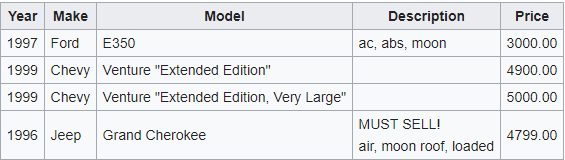
\includegraphics[width=0.6\textwidth]{figures/4/1174083/Teori/contohCSV1.png}}
		\caption{Contoh file}
		\label{Contoh CSV}
		\centerline{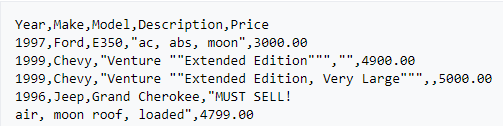
\includegraphics[width=0.6\textwidth]{figures/4/1174083/Teori/contohCSV2.png}}
		\caption{Contoh CSV}
		\label{Contoh CSV2}
	\end{figure}
	
\subsection{Soal 2}	

\textbf{Macam-macam aplikasi CSV}
\begin{enumerate}
\item Program Spreadsheet

Seperti Microsoft Excel, Kspread, Staroffice Calc, OpenOffice Calc, Abacus, Gnumeric, WingZ, XESS.			
\item Texteditor

Seperti Notepad, Notepad++, Sublime, NetBeans, Adobe Dreamweaver, Visual Studio Code, dll 

\end{enumerate}

\subsection{Soal 3}

\textbf{menulis dan membaca file csv}

Sesuai namanya, data atau nilai yang terdapat pada file CSV satu dengan yang lain dipisahkan dengan karakter koma (,). Jika berganti baris, maka itu dianggap record baru. Tentu saja ada kondisi tertentu yang harus dipenuhi agar file Excel bisa disimpan dalam format CSV. Setidaknya ada tiga kondisi utama yang harus dipenuhi, yaitu:
	\begin{itemize}
	\item Data yang diolah di Excel hanya berupa teks atau angka.
	\item Tidak mengandung VBA{Visual Basic for Application}.
	\item Hanya terdiri dari satu sheet.
	\end{itemize}

Langkah untuk menyimpan file ke dalam format CSV cukup mudah, yaitu dengan memilih File $>$ Save As (Excel 2003 atau sebelumnya) atau dengan mengklik Microsoft Office Button $>$ Save As pada Excel 2007. Setelah itu pada kotak dialog yang muncul, pilihlah format CSV (Comma delimited) (*.csv) melalui drop-down Save as type.

\subsection{Soal 4}

\textbf{Sejarah library CSV}

CSV digunakan pada tahun 1983. untuk komputer Osborne Executive, yang membundel spreadsheet SuperCalc, mendokumentasikan konvensi kutipan CSV yang memungkinkan string mengandung koma yang disematkan, tetapi manual tersebut tidak menentukan konvensi untuk menanamkan tanda kutip dalam string yang dikutip. Daftar nilai yang dipisahkan dengan koma lebih mudah untuk diketik daripada data yang selaras dengan kolom tetap, dan cenderung menghasilkan hasil yang salah jika suatu nilai dieksekusi satu kolom dari lokasi yang dituju.

\subsection{Soal 5}

\textbf{Sejarah library Pandas}

Pengembangnya ialah Wes McKinney, mulai mengerjakan pandas pada 2008 ketika di AQR Capital Management karena kebutuhan akan alat kinerja tinggi yang fleksibel untuk melakukan analisis kuantitatif pada data keuangan. Sebelum meninggalkan AQR, dia bisa meyakinkan manajemen untuk mengizinkannya membuka sumber perpustakaan. Pegawai AQR lainnya, Chang She, bergabung dengan proyek ini pada 2012 sebagai kontributor utama kedua ke perpustakaan. Pada 2015, pandas menandatangani sebagai proyek NumFOCUS yang disponsori secara fiskal, sebuah badan amal nirlaba 501(c)(3) di Amerika Serikat.

\subsection{Soal 6}

\textbf{Fungsi-fungsi pada library CSV}

\begin{itemize}
\item csv.reader

Berfungsi untuk membaca dan mengembalikan data kedalam variable dari file csv.	Fungsi 	reader dirancang untuk mengambil data pada setiap baris didalam file dan membuat daftar semua 	kolom. Kemudian, tinggal dipilih kolom mana yang diinginkan untuk data variabel.
\lstinputlisting[firstline=12, lastline=24]{src/4/1174083/Teori/1174083_csv.py}

\item csv.writer

Berfungsi untuk menuliskan data dari variable kedalam file csv. Fungsi writer akan membuat objek yang cocok untuk menulis. Untuk mengulang data yang ada di atas baris, gunakan fungsi writerow.
\lstinputlisting[firstline=39, lastline=45]{src/4/1174083/Teori/1174083_csv.py}
	
\item csv.register\textunderscore dialect untuk Mendaftarkan dialect pada csv
\item csv.unregister\textunderscore dialect untuk Menghapus dialect yang diasosiasi dengan nama dari registry dialect
\item csv.list\textunderscore dialects untuk Mengembalikan dialect yang diasosiasi dengan nama
\item csv.field\textunderscore size\textunderscore limit Mengembalikan ukuran field maksimum yang diizinkan oleh parser.
\item csv.DictReader

Berfungsi untuk membaca dan mengembalikan data kedalam variable dictionary dari file csv.
\lstinputlisting[firstline=26, lastline=37]{src/4/1174083/Teori/1174083_csv.py}
\end{itemize}

\subsection{Soal 7}

\textbf{•}

\begin{itemize}
\item pandas.read\textunderscore csv

Berfungsi untuk membaca dan mengembalikan data kedalam format DataFrame dari file csv.
\lstinputlisting[firstline=47, lastline=50]{src/4/1174083/Teori/1174083_csv.py}
\item to\textunderscore csv

Berfungsi untuk mengedit data didalam csv dan menulisnya kedalam file csv
\lstinputlisting[firstline=52, lastline=59]{src/4/1174083/Teori/1174083_csv.py}

\end{itemize}


\subsection{Bukti Screenshoot}
\begin{figure}[H]
	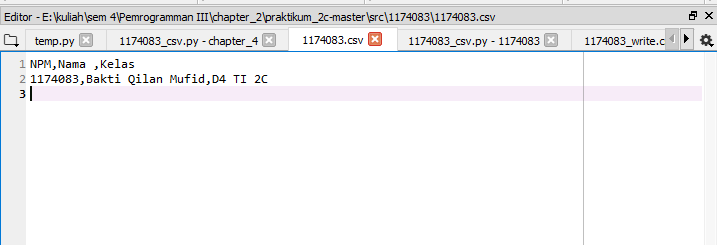
\includegraphics[width=10cm]{figures/4/1174083/Teori/kode_teori_1.png}
	\centering
\end{figure}

\begin{figure}[H]
	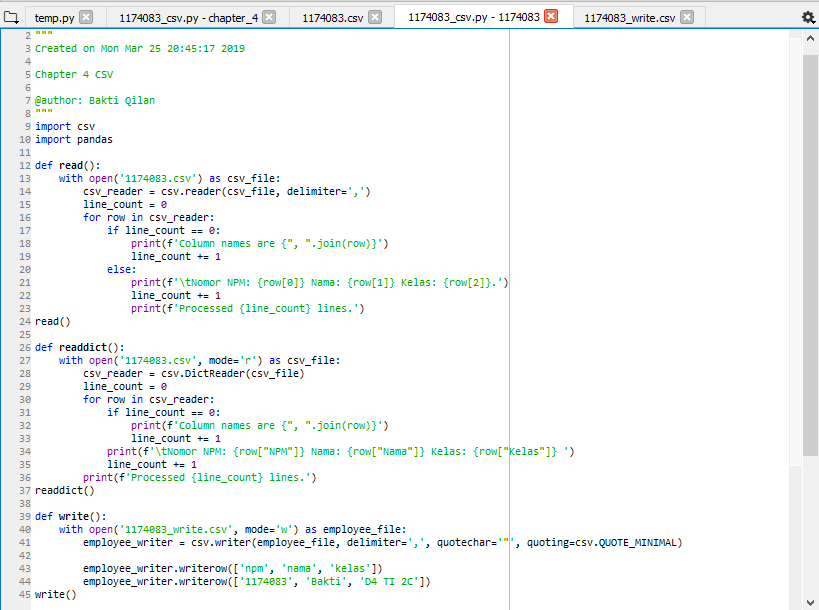
\includegraphics[width=10cm]{figures/4/1174083/Teori/kode_teori_2.png}
	\centering
\end{figure}

\begin{figure}[H]
	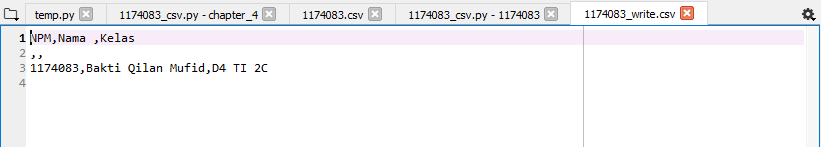
\includegraphics[width=10cm]{figures/4/1174083/Teori/kode_teori_3.png}
	\centering
\end{figure}

\begin{figure}[H]
	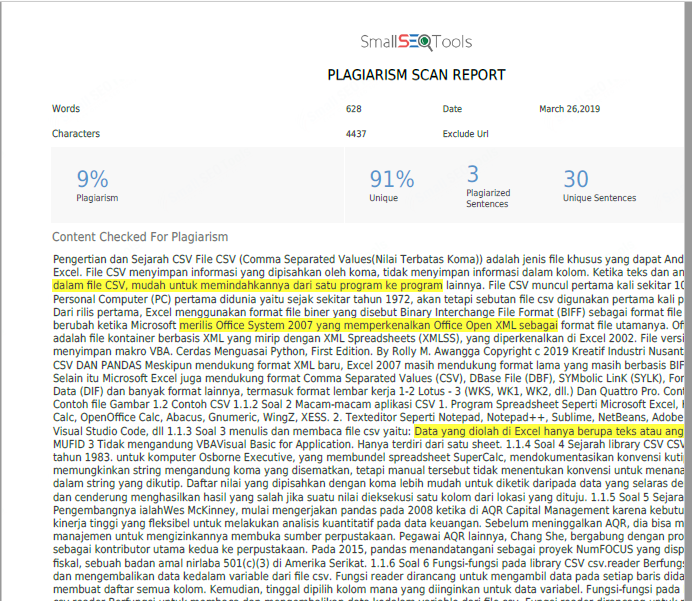
\includegraphics[width=10cm]{figures/4/1174083/Teori/plagiarisme.png}
	\centering	
	\caption{Cek Plagiat}
\end{figure}

%%%%%%%%%%%%%%%%%%%%%%%%%%%%%%%%%%%%%%%%%%%%%%%%%%%%%%%%%%%%%%%%%%%%%%%%%%%%%

\section{Muhammad Reza Syachrani / 1174084}
\subsection{Pemahaman Teori}
\begin{enumerate}
    \item CSV adalah Comma Separated Values suatu format data dalam basis data di mana setiap record dipisahkan dengan tanda koma (,) atau titik koma (;). Selain sederhana, format ini dapat dibuka dengan berbagai text-editor seperti Notepad, Wordpad, bahkan MS Excel.
    \par File CSV (Nilai Berbatas Koma) adalah tipe file khusus yang dapat Anda buat atau edit di Excel. File CSV menyimpan informasi yang dipisahkan oleh koma, bukan menyimpan informasi dalam kolom. Saat teks dan angka disimpan dalam file CSV, mudah untuk memindahkannya dari satu program ke program lain. Misalnya, Anda dapat mengekspor kontak dari Google ke dalam file CSV, kemudian mengimpornya ke Outlook.
    \item Aplikasi-aplikasi yang bisa menciptakan file CSV antara lain adalah notepad++, visual studio code, atom, sublime, excell, google spreadshare, dan LibreOfficecalc.
    \item Cara menulis file csv di excel atau spreadsheet
    \begin{enumerate}
        \item Buat dokumen baru di Excel.
        \item Tambahkan judul kolom untuk setiap informasi yang mau dicatat (misalnya nama, alamat email, nomor telepon, dan ulang tahun), selanjutnya ketikkan informasi dalam kolom yang sesuai.
        \item Setelah selesai, Pilih File > Simpan Sebagai.
        \item Gunakan kotak menurun untuk memilih CSV (Berbatas koma) (*.csv), beri nama pada file, lalu pilih Simpan
    \end{enumerate}
    \par Sedangkan cara membaca file csv di excel atau spreadsheet
    \begin{enumerate}
        \item klik data - get external data - form text
        \item Text Import Wizard, arahkan pada file csv lalu Open
        \item Setelah File terbuka, akan muncul Text Import Wizard.
        \item Pilih Delimited, Kemudian Next (Di sini, bisa juga menentukan baris awal yang akan di import)
        \item Centrang pada Tab dan Comma (Atau sesuai pengaturan File Anda) lalu Next.
        \item Atur Format data pada tiap kolom yang tampil dan klik Finish
    \end{enumerate}
    \item Sejarah Library CSV  dibuat untuk mepermudah mengolah data dan mempermudah untuk melakukan export dan import file CSV.
    \item Sejarah library pandas dibuat untuk bahasa pemograman python agar bisa bersaing dengan  R dan matlab, yang digunakan untuk mengolah banyak data , keperluan big data, data mining, dan data science.
    \item fungsi-fungsi yang terdapat di library CSV
    \begin{itemize}
        \item Reading CSV
        \par csv.reader digunakan untuk Membaca dari file CSV dilakukan menggunakan objek pembaca. File CSV dibuka sebagai file teks dengan fungsi open () built-in Python, yang mengembalikan objek file.
        \item Writing CSV
        \par csv.writer digunakan untuk dapat menulis ke file CSV.
    \end{itemize}
    \item fungsi-fungsi yang terdapat di library pandas
    \begin{itemize}
        \item Reading CSV
        \par pandas.read\_csv digunakan untuk membuka, menganalisis, dan membaca file CSV yang disediakan, dan menyimpan data dalam DataFrame.
        \item Writing CSV
        \par  Menulis DataFrame ke file CSV semudah membaca. contoh membuat variabel df yang menggunakan pandas.read\_csv setelah itu menambahkan fungsi to\_csv () pada varibel df untuk memberikan nama file.
    \end{itemize}
    
\end{enumerate}
\textbf{ Plagiarism}

\begin{figure}[H]
 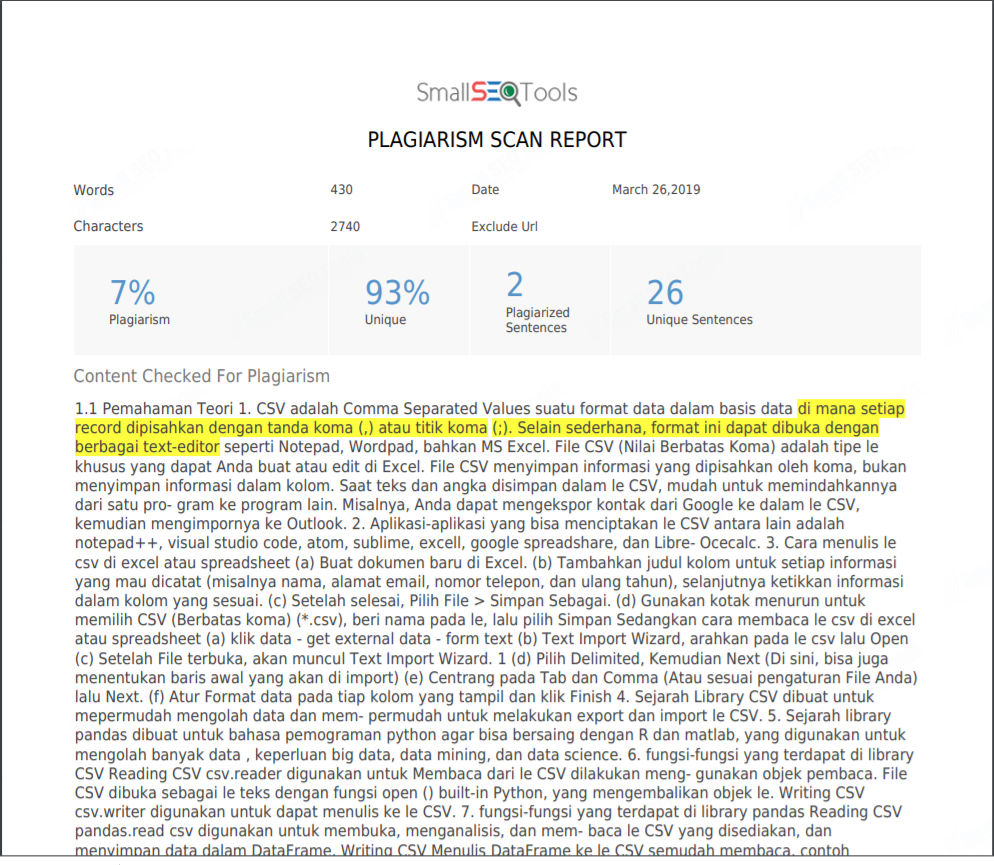
\includegraphics[width=10cm]{figures/4/1174084/Teori/c4_1.png}
 \centering
\end{figure}

%%%%%%%%%%%%%%%%%%%%%%%%%%%%%%%%%%%%%%%%%%%%%%%%%%%%%%%%%%%%%%%%%%%%%%%%%%%%%%
\section{Advent Nopele Olansi Damiahan Sihite}
\subsection{Soal 1}
\textbf{Pengenalan CSV}

Comma Separated Values (CSV) adalah suatu format data yang di mana setiap bagian data dipisahkan dengan tanda koma (,). Format CSV biasanya berfungsi untuk menukar atau mengonversi data ke format lainnya 
%\cite{shafranovich2005common}.

\textbf{Sejarah Format CSV}

IBM Fortran (level H extended) compiler di bawah OS/360 mendukung format CSV pada tahun 1972. FORTRAN 77 mendefinisakan penulisannya dimana input atau output penulisannya menggunakan tanda koma atau spasi untuk pembatas antar data dan penulisan tersebut telah disetujui pada tahun 1978.

Osborne Executive computer yang mengembangkan SuperCalc spreadsheet pada tahun 1983 membuat konvensi kutipan CSV yang memungkinkan string mengandung koma.

Inisiatif standardisasi utama - mentransformasikan "definisi fuzzy de facto" menjadi definisi yang lebih tepat dan de jure - adalah pada tahun 2005, dengan RFC4180, mendefinisikan CSV sebagai Tipe Konten MIME. Kemudian, pada 2013, beberapa kekurangan RFC4180 ditangani oleh rekomendasi W3C.

Pada 2014 IETF menerbitkan RFC7111 yang menjelaskan aplikasi fragmen URI pada dokumen CSV. RFC7111 menentukan bagaimana rentang baris, kolom, dan sel dapat dipilih dari dokumen CSV menggunakan indeks posisi.

Pada 2015 W3C, dalam upaya meningkatkan CSV dengan semantik formal, mempublikasikan draft rekomendasi pertama untuk standar metadata CSV, yang dimulai sebagai rekomendasi pada bulan Desember tahun yang sama.

\textbf{Contoh penggunaan format CSV}

\lstinputlisting[caption = Contoh penggunaan format CSV., firstline=1, lastline=3]{src/4/1174089/Teori/teori.csv}

\subsection{Soal 2}
Aplikasi-aplikasi yang dapat menciptkan file csv, yaitu:

\begin{enumerate}
	\item Editor teks (Notepad, Sublime, Atom, dan lain-lain)
	\item Spreadsheet (Microsoft Excel dan lain-lain)
\end{enumerate}

\subsection{Soal 3}
Cara menulis dan membaca file csv di excel atau spreadsheet, sebagai berikut:

\textbf{Menulis File CSV}

\begin{enumerate}
	\item Pertama silahkan buka aplikasi Excel dengan cara klik ''Start'', cari Excel, kemudian tekan Enter.
	
	\begin{figure}[H]
		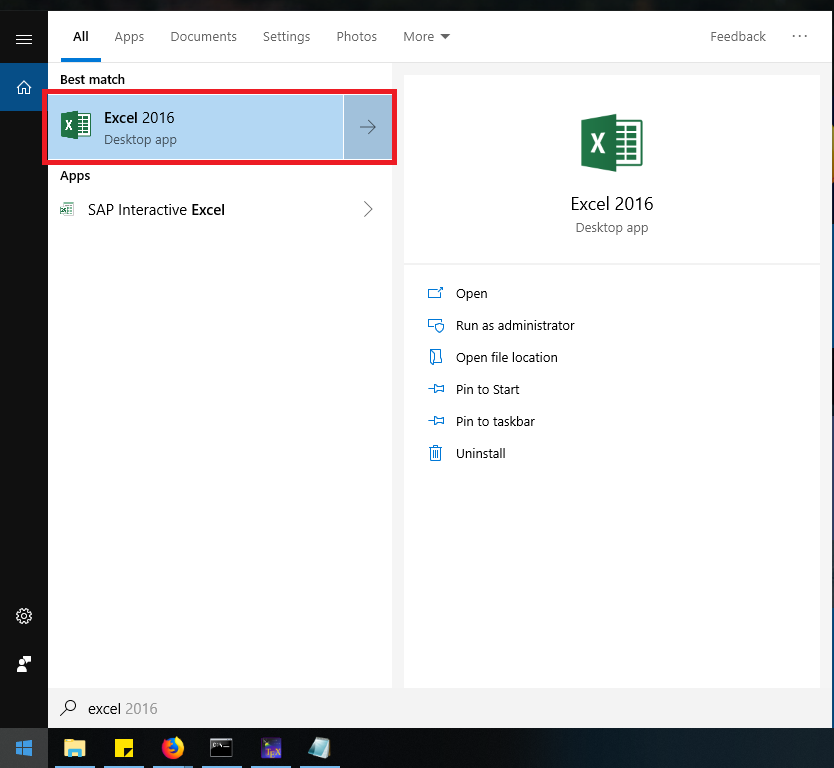
\includegraphics[width=9cm]{figures/4/1174089/Teori/t1.png}
		\centering
	\end{figure}
	
	\item Setelah aplikasi terbuka silahkan klik ''Blank Workbook''.
	
	\begin{figure}[H]
		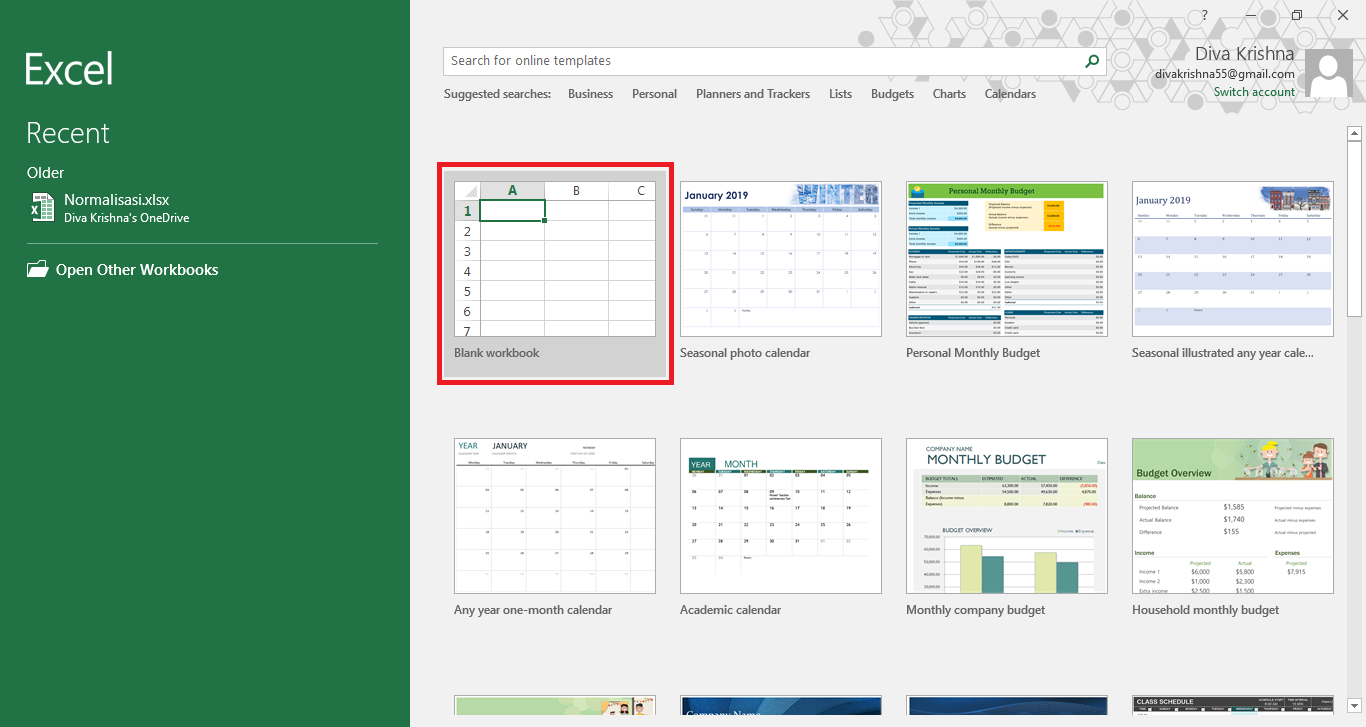
\includegraphics[width=10cm]{figures/4/1174089/Teori/t2.png}
		\centering
	\end{figure}
	
	\item Kemudian isi sesuai dengan data yang ingin dibuat.
	
	\begin{figure}[H]
		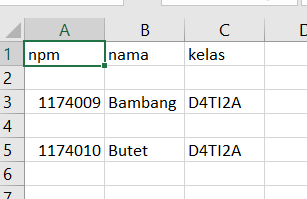
\includegraphics[width=10cm]{figures/4/1174089/Teori/t3.png}
		\centering
	\end{figure}
	
	\item Setelah selesai dibuat, silahkan simpan file tersebut dengan cara mengklik ''File'', lalu klik ''Save''.
	
	\begin{figure}[H]
		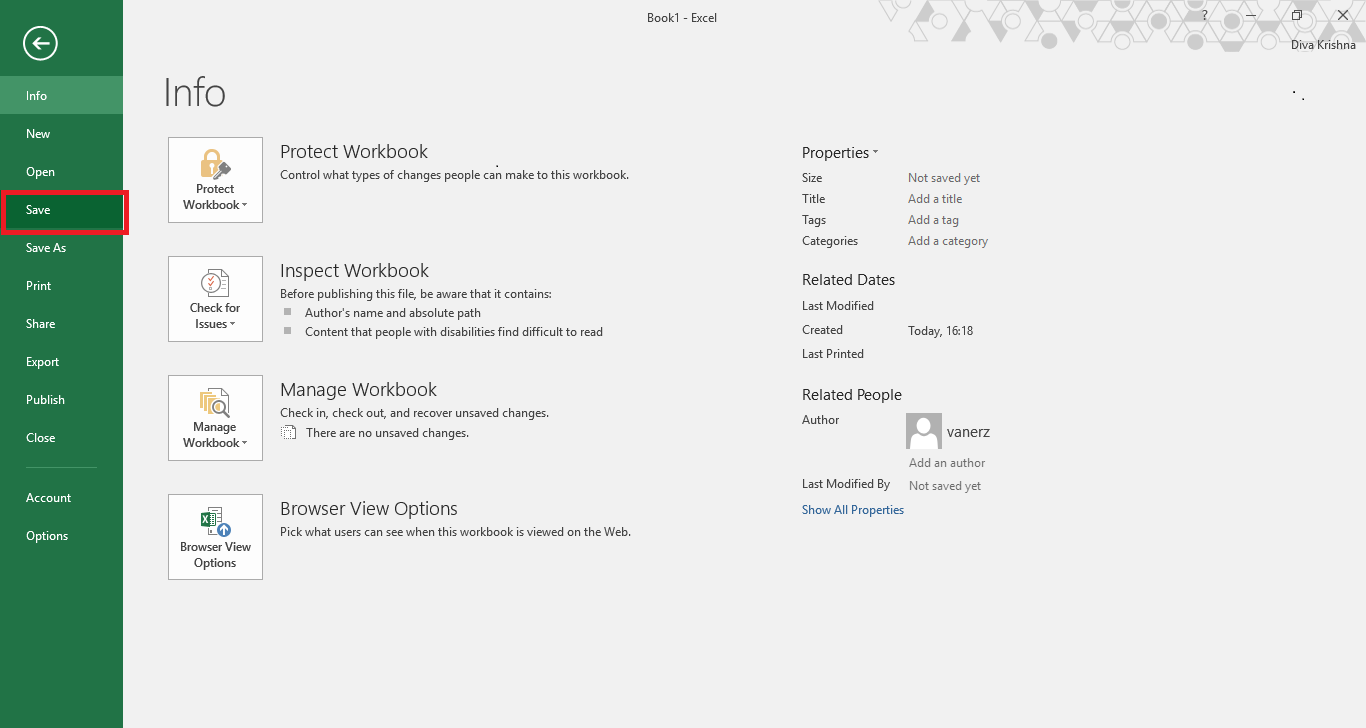
\includegraphics[width=10cm]{figures/4/1174089/Teori/t4.png}
		\centering
	\end{figure}
	
	\item Kemudian isi kolom ''File name'' dengan nama file anda dan kolom ''Save as type'' pilih yang berekstensi .csv.
	
	\begin{figure}[H]
		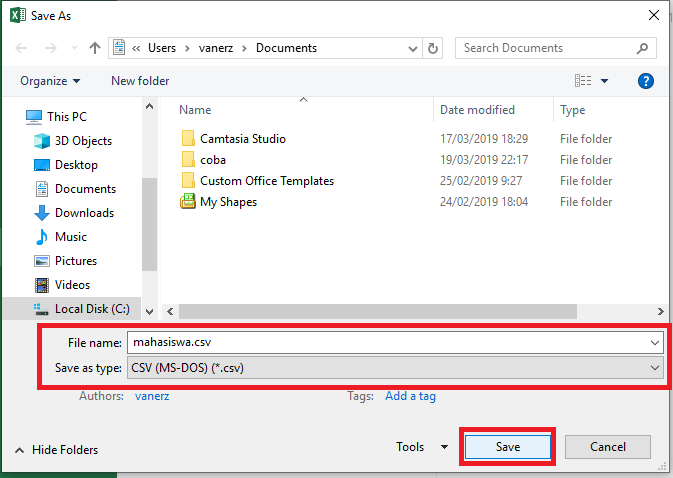
\includegraphics[width=9cm]{figures/4/1174089/Teori/t5.png}
		\centering
	\end{figure}
	
	\item Lalu tinggal klik ''Yes''.
	
	\begin{figure}[H]
		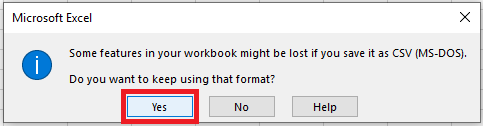
\includegraphics[width=7cm]{figures/4/1174089/Teori/t6.png}
		\centering
	\end{figure}
	
	\item Kemudian file yang Anda telah terbuat tadi tersimpan dengan ekstensi .csv. Untuk melihat isi filenya tinggal klik dua kali pada file tersebut.
	
	\begin{figure}[H]
		
\includegraphics[width=10cm]{figures/4/1174089/Teori/t8.png}
		\centering
	\end{figure}
	
	\item Berikut ini adalah isi dari file yang tadi Anda buat.
	
	\begin{figure}[H]
		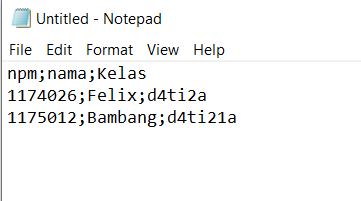
\includegraphics[width=8cm]{figures/4/1174089/Teori/t7.png}
		\centering
	\end{figure}
\end{enumerate}

\textbf{Melihat File CSV di Excel atau Spreadsheet}

\begin{enumerate}
	\item Pertama klik dua kali pada file yang yang berekstensi CSV.
	
	\begin{figure}[H]
		
\includegraphics[width=10cm]{figures/4/1174089/Teori/t8.png}
		\centering
	\end{figure}
	
	\item Kemudian file akan terbuka secara otomatis di aplikasi Excel atau spreadsheet.
	
	\begin{figure}[H]
		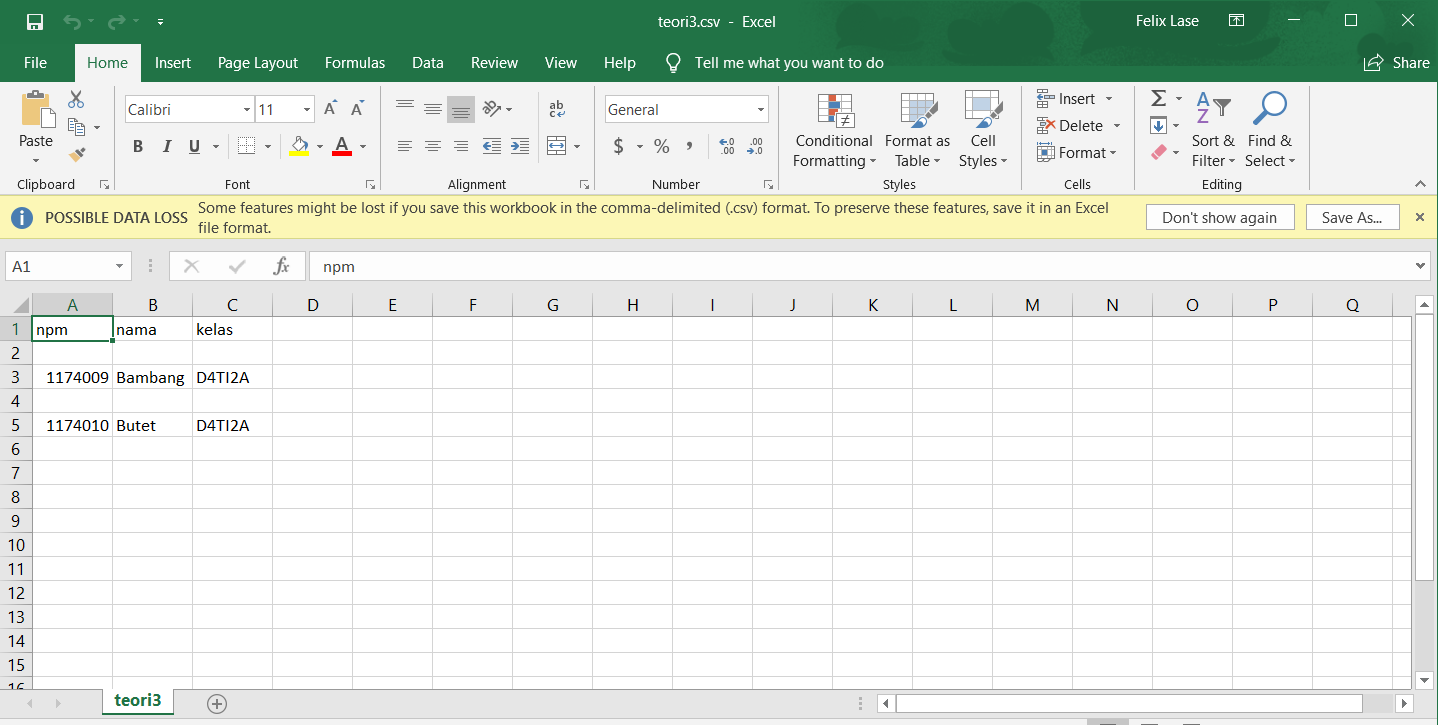
\includegraphics[width=10cm]{figures/4/1174089/Teori/t9.png}
		\centering
	\end{figure}
\end{enumerate}
%%%%%%%%%%%%%%%%%%%%%%%%%%%%%%%%%%%%%%%%%%%%%%%%%%%%%%%%%%%%%%%%%%%%%%%%%%%%%%%%%%%%
\section{Mochamad Arifqi Ramadhan | 1174074}
\subsection{Pengelolaan File CSV (Teori)}
\begin{enumerate}

\item 1. Apa itu fungsi file csv, jelaskan sejarah dan contoh\\
Jawaban :

\begin{itemize}
\item Fungsi File CSV
\end{itemize}

Comma Separated Value (CSV) adalah file teks biasa yang berisi daftar data. File-file ini sering digunakan untuk bertukar data antara aplikasi yang berbeda, selain itu CSV memudahkan penggunanya melakukan penginputan data ke database secara sederhana. CSV bisa digunakan dalam standar file ASCII, di mana setiap record dipisahkan dengan tanda koma atau titik koma.

\begin{itemize}
\item Sejarah 
\end{itemize}

csv muncul pertama kali sekitar 10 tahun sebelum Personal Computer (PC)  pertama didunia, yaitu sejak sekitar tahun 1972, akan tetapi sebutan file csv digunakan pertama kali pada tahun 1983.

\begin{itemize}
\item Contoh file csv
\begin{verbatim}
Nama, Email, kelas.
Arifqi, arifqiramadhan890@gmail.com, D4 TI-2C.
\end{verbatim}
\end{itemize}

\item 2.  Aplikasi yang dapat membuat file csv?\\
Jawaban :

\begin{itemize}
\item Notepad ++
\item Microsoft Excel
\item  Google Spreadsheet
\item Text Editor dan program spreadsheet  lainnya
\end{itemize}

\item 3. Cara menulis dan membaca file csv di excel atau spreadsheet\\
Jawaban :

\begin{itemize}
\item Cara Menulis file csv di excel atau spreadsheet
\end{itemize}
Berikut adalah kode untuk menulis file CSV dengan menggunakan built-in module csv yang dimiliki Python

\begin{verbatim}
	\item Buka Microsoft Excel  lalu buat dokumen baru
	\item Masukkan data sesuai dengan kebutuhan, data paling atas akan menjadi header dari file csv
	\item Setelah memasukkan data, klik file lalu klik Save As
	\item Pilih Browse dan pilih tempat menyimpannya akan dimana
	\item Masukkan nama filenya dan save as dengan memilih type filnya CSV (nama file.csv)
\end{verbatim}

\begin{itemize}
\item Cara membaca file csv di excel atau spreadsheet
\end{itemize}

\begin{verbatim}
CSV file to excel, cara pertama bisa dengan klik dua kali file .csv untuk membukanya di Excel secara default. Jika tidak terbuka dunakan cara lain dengan  mengklik kanan file CSV dan pilih Open With > Excel. 
Dan cara ke dua dengan membuka aplikasi Microsoft Excel, kemudian pilih menu Open, kemudian cari tempat file csv yang ingin dibuka, lalu pilih Open File csv sudah berhasil dibaca menggunakan Microsoft Excel

\item Jika setelah membuka file CSV ternyata semua teksnya berada dalam satu kolom tidak dipisahkan dengan koma ataupun karakter lainnya, Anda dapat membuka file dari dalam Microsoft Excel (seperti yang disebutkan di atas) akan memunculkan Teks Wizard Impor pembukaan. Itu meminta Anda untuk memilih bagaimana teks dipisahkan. Pilih opsi Delimited, maka pada layar kemudian pilih opsi Comma. Hal ini akan menghasilkan teks yang terpisahkan dengan koma menjadi terpisahkan dengan kolom-kolom tersendiri.
\end{verbatim}

\item 4. Sejarah library csv\\
Jawaban :\\
Comma-separated values (CSV) adalah format data yang memberi tanggal lebih awal pada komputer pribadi lebih dari satu dekade: kompiler IBM Fortran (level H extended) di bawah OS / 360 mendukungnya pada tahun 1972. [6] Input / output daftar-diarahkan ("bentuk bebas") didefinisikan dalam FORTRAN 77, disetujui pada tahun 1978. Input yang diarahkan daftar menggunakan koma atau spasi untuk pembatas, sehingga string karakter yang tidak dikutip tidak dapat mengandung koma atau spasi.

\item 5. Sejarah library pandas\\
Jawaban :\\
Pada akhir tahun 2009 pandas menjadi Open Sourced, dimana disupport oleh banyak komunitas atau individu di dunia untuk mengembangkan pandas. Sejak tahun 2015, pandas menjadi NumFOCUS proyek sponsor, ini juga membantu suksesnya pengembangan dari pandas itu sendiri. pandas merupakan struktur data dan data analysis tools untuk bahasa pemrograman Python, dan merupakan BSD-licensed library yang menjadikannya memiliki performa yang tinggi.


\item 6. Jelaskan  fungsi-fungsi yang terdapat di library csv\\
Jawaban :\\
Library CSV memiliki 2 fungsi, yaitu :

\begin{itemize}
\item Membaca file (csv reader)
\end{itemize}
Berfungsi untuk membaca dan mengembalikan data kedalam variable dari file csv.
\begin{itemize}
\item Menulis file (csv writer)
\end{itemize}
Berfungsi untuk menuliskan data dari variable kedalam file csv.

\item 7. Jelaskan  fungsi-fungsi yang terdapat di library pandas\\
Jawaban :\\
Library pandas memiliki fungsi penting seperti menyelaraskan data untuk perbandingan dan penggabungan set data, penanganan data yang hilang, dll, itu telah menjadi sebuah library untuk pemrosesan data tingkat tinggi dalam Python (yaitu statistik).

\end{enumerate}

\textbf{Screenshoot Check Plagiarisme}

\begin{figure}[H]
 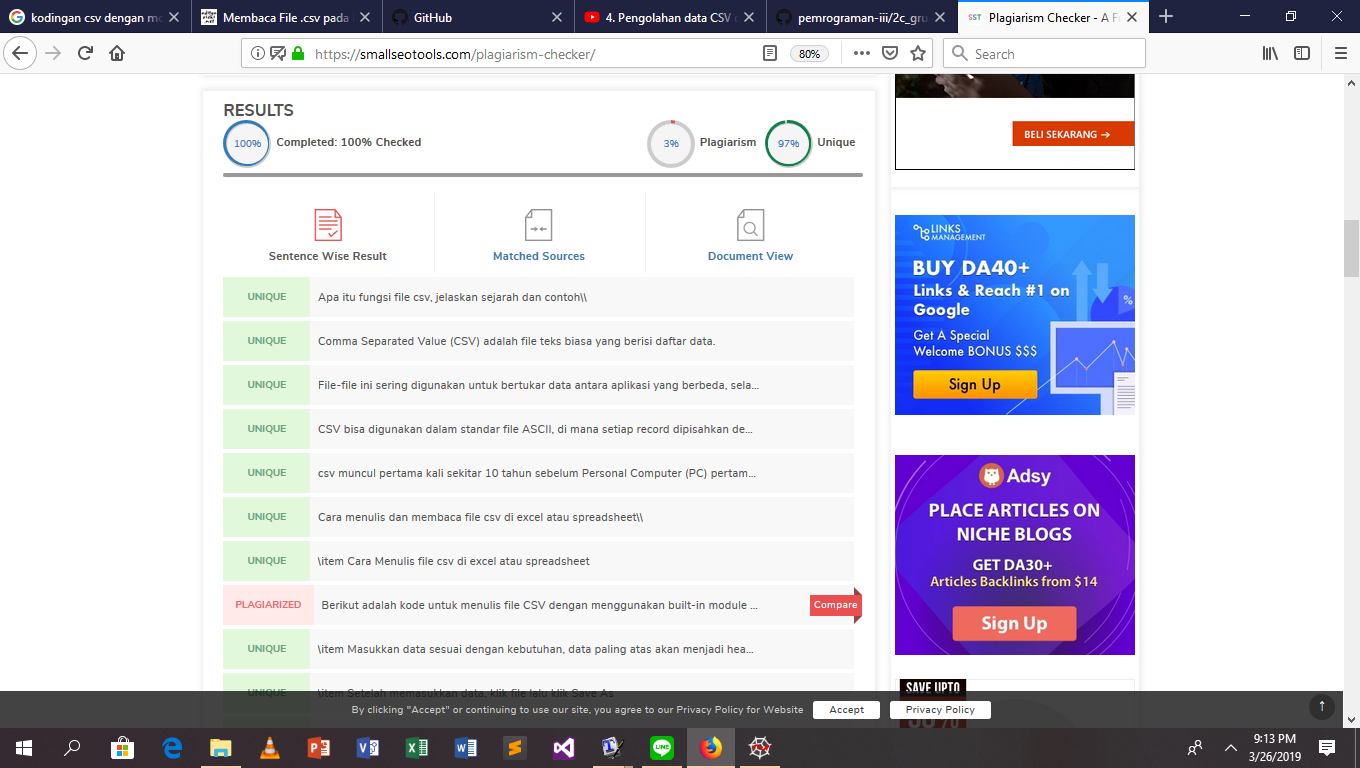
\includegraphics[width=5cm]{figures/4/1174074/Teori/plagiarisme.png}
 \centering
\end{figure}
%%%%%%%%%%%%%%%%%%%%%%%%%%%%%%%%%%%%%%%%%%%%%%%%%%%%%%%%%%%%%%%%%%%%%%%%%%%%%%%%%%%%%%%%%%%%%%%%%%%%%%%%%%
%PRAKTEK
%\chapter{Praktek Library CSV dan Pandas}
%\section{Ilham Muhammad Ariq D4TI2C 1174087}
\subsection{Keterampilan Pemrograman}
\begin{enumerate}
    \item Buatlah  fungsi  (file  terpisah/library  dengan  nama  \verb|NPM_csv.py|)  untuk  membuka file csv dengan lib csv mode list.
    
    \lstinputlisting[firstline=8, lastline=14]{src/4/1174087/Praktek/1174087_csv.py}

    \item Buatlah  fungsi  (file  terpisah/library  dengan  nama  \verb|NPM_csv.py|)  untuk  membuka file csv dengan lib csv mode dictionary.
   	
   	\lstinputlisting[firstline=16, lastline=20]{src/4/1174087/Praktek/1174087_csv.py}

	\item Buatlah fungsi (file terpisah/library dengan nama \verb|NPM_pandas.py|) untuk membuka file csv dengan lib pandas mode list.
	
	\lstinputlisting[firstline=7, lastline=11]{src/4/1174087/Praktek/1174087_pandas.py}
		
	\item Buatlah fungsi (file terpisah/library dengan nama \verb|NPM_pandas.py| untuk membuka file csv dengan lib pandas mode dictionary.

	\lstinputlisting[firstline=13, lastline=16]{src/4/1174087/Praktek/1174087_pandas.py}

	\item Buat fungsi baru di \verb|NPM_pandas.py| untuk mengubah format tanggal menjadi standar dataframe.

	\lstinputlisting[firstline=25, lastline=27]{src/4/1174087/Praktek/1174087_pandas.py}

	\item Buat fungsi baru di \verb|NPM_pandas.py| untuk mengubah index kolom.
	
	\lstinputlisting[firstline=29, lastline=32]{src/4/1174087/Praktek/1174087_pandas.py}
	
	\item Buat fungsi baru di \verb|NPM_pandas.py| untuk mengubah atribut atau nama kolom.
	
	\lstinputlisting[firstline=34, lastline=37]{src/4/1174087/Praktek/1174087_pandas.py}
	
	\item Buat program main.py yang menggunakan library \verb|NPM_csv.py| yang membuat dan membaca file csv.
	
	\lstinputlisting[firstline=8, lastline=15]{src/4/1174087/Praktek/main.py}
	
	\item Buat program main2.py yang menggunakan library \verb|NPM_pandas.py| yang membuat dan membaca file csv.

	\lstinputlisting[firstline=8, lastline=12]{src/4/1174087/Praktek/main2.py}
\end{enumerate} 

\subsection{Keterampilan Penanganan Error}

\begin{enumerate}
	\item Tuliskan peringatan error yang didapat dari mengerjakan praktek ketiga ini,
dan jelaskan cara penanganan error tersebut. dan Buatlah satu fungsi yang
menggunakan gunakan try except untuk menanggulangi error tersebut.

	\lstinputlisting[firstline=7, lastline=16]{src/4/1174087/Praktek/error.py}
	
	\par NameError adalah exception yang terjadi saat kode melakukan eksekusi terhadap local name atau global name yang tidak terdefinisi. Misalnya saat menjumlahkan variable yang tidak didefinisikan, memanggil function yang tidak ada, dan lain-lain.
	
\end{enumerate}

\textbf{Screenshoot Kode Program Python}

\begin{figure}[H]
 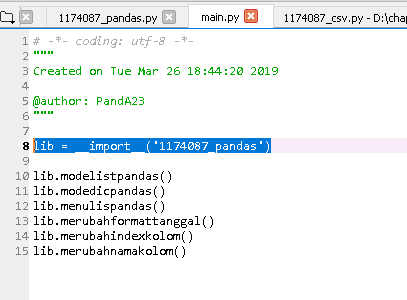
\includegraphics[width=5cm]{figures/4/1174087/Praktek/main.png}
 \centering
\end{figure}

\begin{figure}[H]
 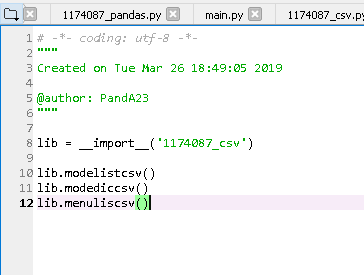
\includegraphics[width=5cm]{figures/4/1174087/Praktek/main2.png}
 \centering
\end{figure}

\begin{figure}[H]
 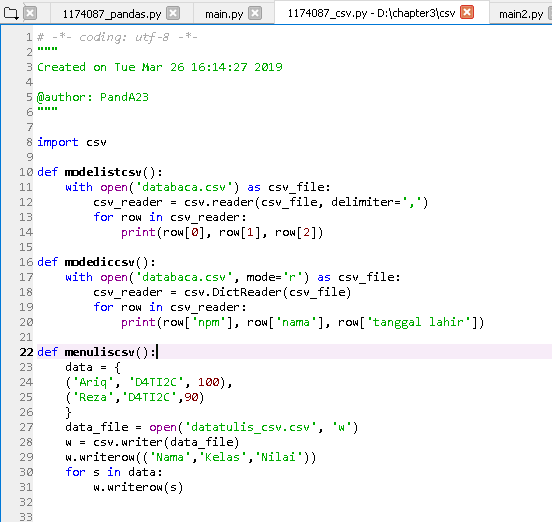
\includegraphics[width=5cm]{figures/4/1174087/Praktek/1174087_csv.png}
 \centering
\end{figure}

\begin{figure}[H]
 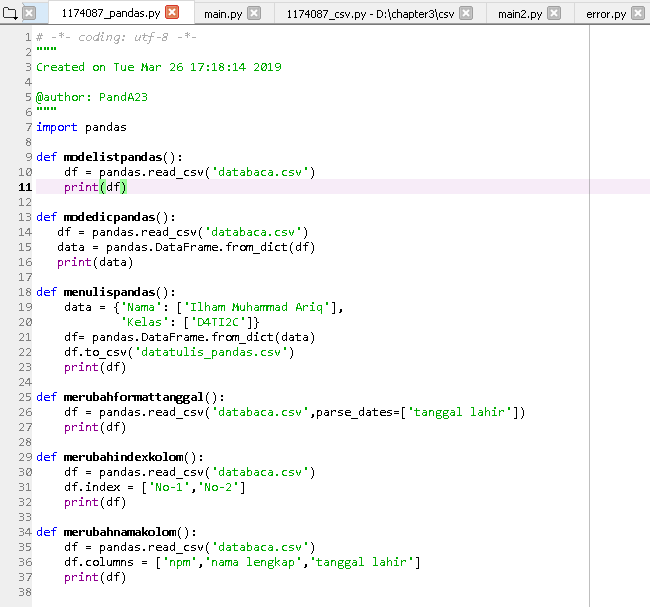
\includegraphics[width=5cm]{figures/4/1174087/Praktek/1174087_pandas.png}
 \centering
\end{figure}

\begin{figure}[H]
 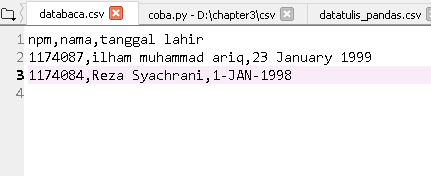
\includegraphics[width=5cm]{figures/4/1174087/Praktek/databaca.png}
 \centering
\end{figure}

\begin{figure}[H]
 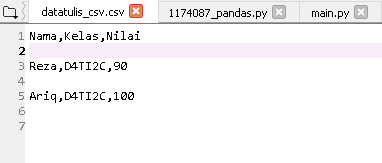
\includegraphics[width=5cm]{figures/4/1174087/Praktek/datatulis_csv.png}
 \centering
\end{figure}

\begin{figure}[H]
 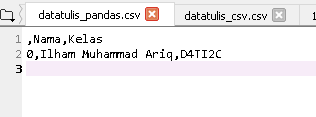
\includegraphics[width=5cm]{figures/4/1174087/Praktek/datatulis_pandas.png}
 \centering
\end{figure}

\begin{figure}[H]
 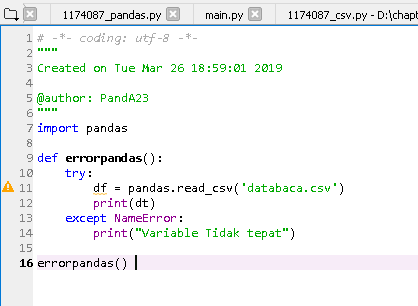
\includegraphics[width=5cm]{figures/4/1174087/Praktek/error.png}
 \centering
\end{figure}

%%%%%%%%%%%%%%%%%%%%%%%%%%%%%%%%%%%%%%%%%%%%%%%%%%%%%%%%%%%%%%%%%%%%%%%%%%%%%%%%%%%%%%%%%%%%%%%%%%%%%%%%%%%%%%%%%%%%%%
\section{Dini Permata Putri | 1174053}
\subsection{Keterampilan Pemrograman}
\begin{enumerate}
\item Buatlah  fungsi  (file  terpisah/library  dengan  nama  NPMcsv.py)  untuk  membuka file csv dengan lib csv mode list.


	\lstinputlisting[firstline=10, lastline=15]{src/4/1174053/Praktek/1174053csv.py}

	\item Buatlah  fungsi  (file  terpisah/library  dengan  nama  NPMcsv.py)  untuk  membuka file csv dengan lib csv mode dictionary.

	\lstinputlisting[firstline=17, lastline=22]{src/4/1174053/Praktek/1174053csv.py}

	\item Buatlah fungsi (file terpisah/library dengan nama NPMpandas.py) untuk membuka file csv dengan lib pandas mode list.

	\lstinputlisting[firstline=10, lastline=13]{src/4/1174053/Praktek/1174053pandas.py}

	\item Buatlah fungsi (file terpisah/library dengan nama NPMpandas.py) untuk membuka file csv dengan lib pandas mode dictionary.

	\lstinputlisting[firstline=10, lastline=13]{src/4/1174053/Praktek/1174053pandas.py}

	\item  Buat fungsi baru di NPMpandas.py untuk mengubah format tanggal menjadi standar dataframe.

	\lstinputlisting[firstline=15, lastline=19]{src/4/1174053/Praktek/1174053pandas.py}

	\item Buat fungsi baru di NPMpandas.py untuk mengubah index kolom.

	\lstinputlisting[firstline=21, lastline=24]{src/4/1174053/Praktek/1174053pandas.py}

	\item Buat fungsi baru di NPMpandas.py untuk mengubah atribut atau nama kolom.

	\lstinputlisting[firstline=26, lastline=30]{src/4/1174053/Praktek/1174053pandas.py}

	\item Buat program main.py yang menggunakan library NPMcsv.py yang membuat dan membaca file csv.

	\lstinputlisting[firstline=8, lastline=13]{src/4/1174053/Praktek/main.py}

	\item Buat program main2.py yang menggunakan library NPMpandas.py yang membuat dan membaca file csv.

	\lstinputlisting[firstline=8, lastline=13]{src/4/1174053/Praktek/main2.py}
\end{enumerate}

\subsection{Penanganan Error}
Peringatan error di praktek keempat ini, yaitu:
	\begin{itemize}
		\item Syntax Errors
		Syntax Error, adalah kesalahan yang disebabkan oleh kesalahan tata cara penulisan tanda baca, kesalahan pemakaian operator dan nilai. Kesalahan jenis ini akan dengan mudah dideteksi oleh kompiler maupun interpreter.

		\item Name Error
		NameError adalah exception yang terjadi saat kode melakukan eksekusi terhadap local name atau global name yang tidak terdefinisi. Misalnya saat menjumlahkan variable yang tidak didefinisikan, memanggil function yang tidak ada, dan lain-lain.

		\item Type Error
		TypeError adalah exception yang akan terjadi apabila pada saat dilakukannya eksekusi terhadap suatu operasi atau fungsi dengan type object yang tidak sesuai. Solusi dari error ini adalah mengkoversi varibelnya sesuai dengan tipe data yang akan digunakan.
	

	\item Fungsi yang menggunakan try except
	\lstinputlisting[firstline=55, lastline=67]{src/4/1174053/Praktek/1174053.py}
\end{itemize}


%%%%%%%%%%%%%%%%%%%%%%%%%%%%%%%%%%%%%%%%%%%%%%%%%%%%%%%%%%%%%%%%%%%%%%%%%%%%%%%%%%%%%%%%%%%%%%%%%%
\section{Bakti Qilan Mufid | 1174083}
\subsection{Soal 1}
Jawaban soal ke-1

\lstinputlisting[caption =  Fungsi untuk membuka file CSV dengan lib CSV mode list.,firstline=11, lastline=16]{src/4/1174083/Praktek/1174083_csv.py}

\subsection{Soal 2}
Jawaban soal ke-2

\lstinputlisting[caption =  Fungsi untuk membuka file CSV dengan lib CSV mode dictionary., firstline=18, lastline=23]{src/4/1174083/Praktek/1174083_csv.py}

\subsection{Soal 3}
Jawaban soal ke-3

\lstinputlisting[caption =  Fungsi untuk membuka file CSV dengan lib Pandas mode list., firstline=11, lastline=14]{src/4/1174083/Praktek/1174083_pandas.py}

\subsection{Soal 4}
Jawaban soal ke-4

\lstinputlisting[caption =  Fungsi untuk membuka file CSV dengan lib Pandas mode dictionary., firstline=16, lastline=20]{src/4/1174083/Praktek/1174083_pandas.py}

\subsection{Soal 5}
Jawaban soal ke-5

\lstinputlisting[caption =  Fungsi untuk mengubah format tanggal menjadi standar dataframe., firstline=22, lastline=25]{src/4/1174083/Praktek/1174083_pandas.py}

\subsection{Soal 6}
Jawaban soal ke-6

\lstinputlisting[caption =  Fungsi untuk mengubah index kolom., firstline=21, lastline=24]{src/4/1174083/Praktek/1174083_pandas.py}

\subsection{Soal 7}
Jawaban soal ke-7

\lstinputlisting[caption =  Fungsi untuk mengubah atribut atau nama kolom., firstline=33, lastline=37]{src/4/1174083/Praktek/1174083_pandas.py}

\subsection{Soal 8}
Jawaban soal ke-8

\lstinputlisting[caption =  Membuat dan membaca file CSV menggunakan library 1174083pandas., firstline=8, lastline=13]{src/4/1174083/Praktek/main.py}

\subsection{Soal 9}
Jawaban soal ke-9

\lstinputlisting[caption = Membuat dan membaca file CSV menggunakan library 1174083pandas., firstline=8, lastline=13]{src/4/1174083/Praktek/main2.py}

\subsection{Bukti Screenshoot}

\begin{figure}[H]
	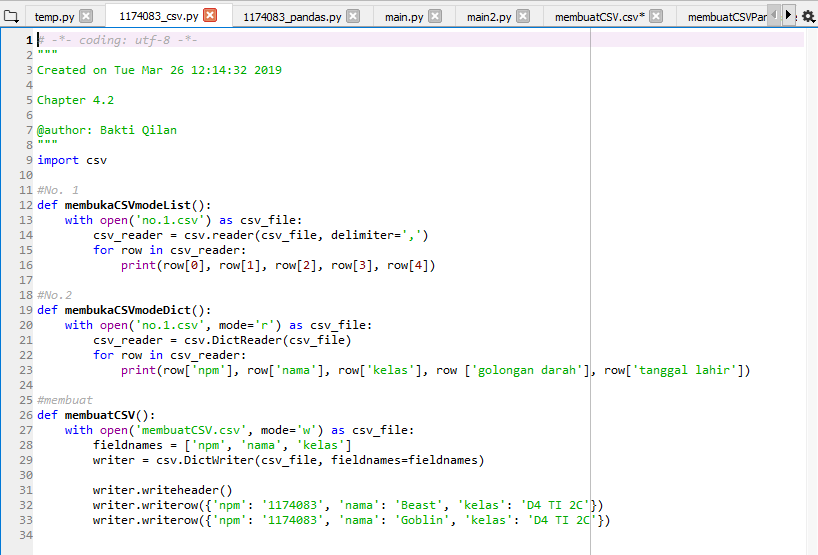
\includegraphics[width=10cm]{figures/4/1174083/Praktek/kode_praktek_1.png}
	\centering
\end{figure}

\begin{figure}[H]
	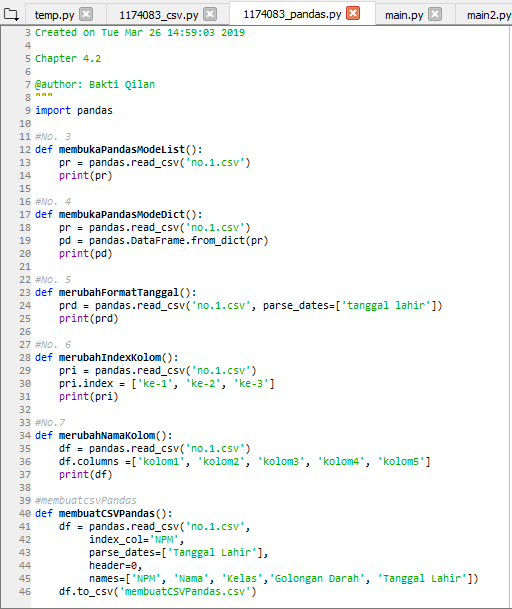
\includegraphics[width=10cm]{figures/4/1174083/Praktek/kode_praktek_2.png}
	\centering
\end{figure}

\begin{figure}[H]
	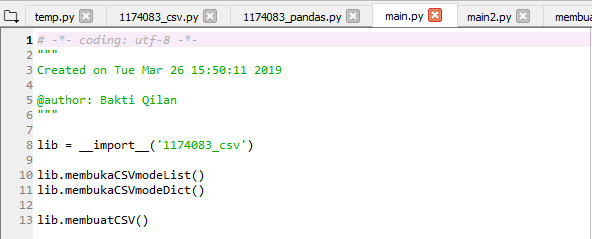
\includegraphics[width=10cm]{figures/4/1174083/Praktek/kode_praktek_3.png}
	\centering
\end{figure}

\begin{figure}[H]
	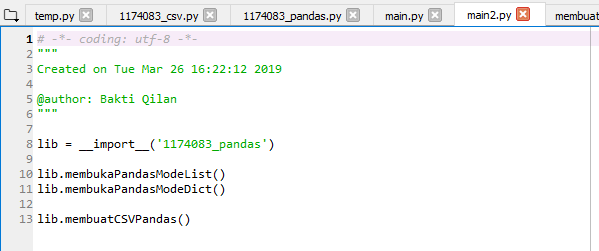
\includegraphics[width=10cm]{figures/4/1174083/Praktek/kode_praktek_4.png}
	\centering
\end{figure}

\begin{figure}[H]
	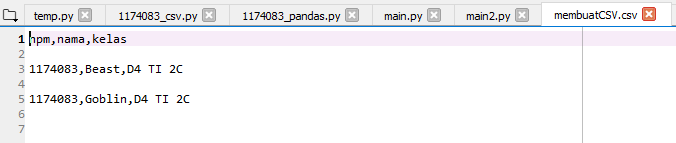
\includegraphics[width=10cm]{figures/4/1174083/Praktek/kode_praktek_5.png}
	\centering
\end{figure}

\begin{figure}[H]
	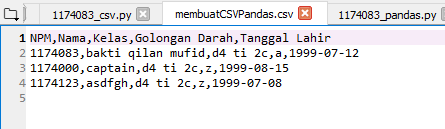
\includegraphics[width=10cm]{figures/4/1174083/Praktek/kode_praktek_6.png}
	\centering
\end{figure}

\begin{figure}[H]
	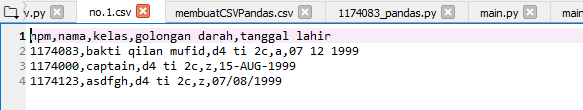
\includegraphics[width=10cm]{figures/4/1174083/Praktek/kode_praktek_7.png}
	\centering
\end{figure}

%TEORI
%\chapter{Komunikasi Perangkat Keras}
%\section{Bakti QIlan Mufid | 1174083}
\subsection{Soal 1}
Apa itu fungsi device manager di windows dan folder /dev di linux.
\begin{itemize}
	\item Device Manager: Device Manager dalam komputer windows, adalah perluasan dari Microsoft Management Console. Device Manager menampilkan seluruh hardware yang bisa di-inisialisasi (dikenali) oleh Windows. dan fungsi dari Device Manager ini ialah dalam mengelola (manage) semua hardware yang terpasang (dan terdeteksi)dalam suatu sistem Windows. Hardware seperti harddisk, kartu VGA, sound, keyboard, perangkat USB dll. akan sangat mudah untuk dikonfigurasi dari dalam Device Manager ini. Device Manager paling sering digunakan untuk pengelolaan driver suatu hardware. Misalnya instalasi driver, uninstal driver, update driver, rollback driver, dan bermacam problem yang berkaitan dengan driver suatu hardware.
	\item folder /dev berisi semua drive harddisk atau hardware seperti modem, CD/DVD/Blu-ray dsb. Hanya saja disini hanya merupakan link dan bukan isi, contohnya hdd partisi 1 ada di /dev/sda1 dan DVD-rom ada di /dev/sr0. untuk melihat isinya, harus dilakukan mounting (mount) terlebih dahulu.
\end{itemize}

\subsection{Soal 2}

Jelaskan langkah-langkah instalasi driver dari arduino UNO di Windows

Berikut ini adalah langkah-langkah instalasi driver dari arduino UNO di Windows
	\begin{itemize}
		\item Pertama pastikan Arduino IDE telah terinstall.
		\item Hubungkan port USB Arduino Uno ke port USB PC.
			\begin{figure}[ht]
				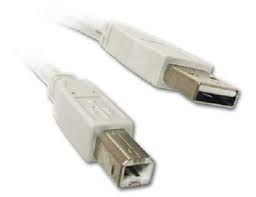
\includegraphics[width=10cm]{figures/5/1174083/Teori/kabel.jpg}
				\centering
				\caption{menghubungkan port.}
			\end{figure}
		\item Lalu pada bagian kanan didesktop PC anda, akan muncul popup “Installing device driver software” seperti pada gambar dibawah ini.
			\begin{figure}[ht]
				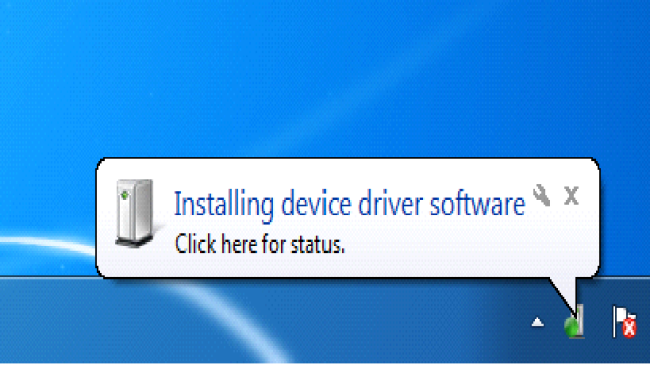
\includegraphics[width=10cm]{figures/5/1174083/Teori/2.png}
				\centering
				\caption{muncul pop up.}
			\end{figure}
		\item SIstem operasi Windows tidak menyediakan driver untuk Arduino Uno seperti yang terlihat pada gambar dibawah ini, lalu proses instalasinya harus dilakukan secara manual.
			\begin{figure}[ht]
				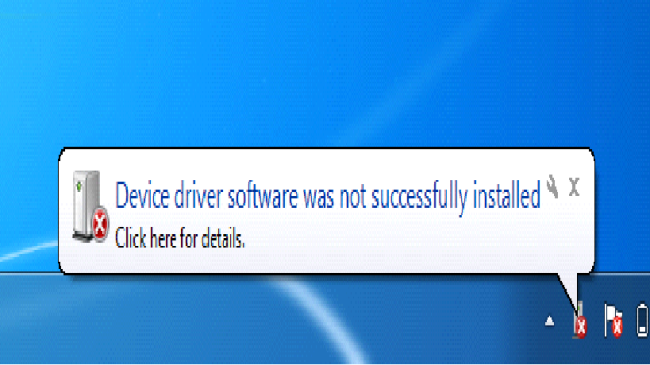
\includegraphics[width=10cm]{figures/5/1174083/Teori/3.png}
				\centering
				\caption{instalasi manual.}
			\end{figure}
		\item Buka Device Manager, caranya pada bagian Search Program and Files lalu ketikkan “device manager” (tanpa tanda petik), perhatikan gambar dibawah ini. Pada bagian Control Panel akan muncul Device Manager, klik untuk menjalankan.
			\begin{figure}[ht]
				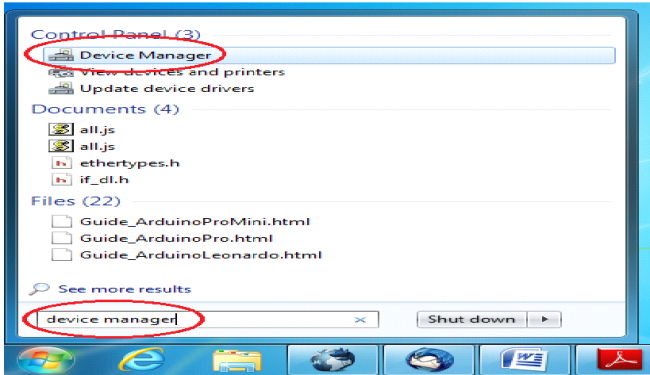
\includegraphics[width=10cm]{figures/5/1174083/Teori/4.png}
				\centering
				\caption{membuka device manager.}
			\end{figure}
		\item Cari Unknown device pada bagian Other device, biasanya terdapat tanda seru berwarna kuning, itu disebabkan karena penginstallan tidak berjalan dengan sempurna.
			\begin{figure}[ht]
				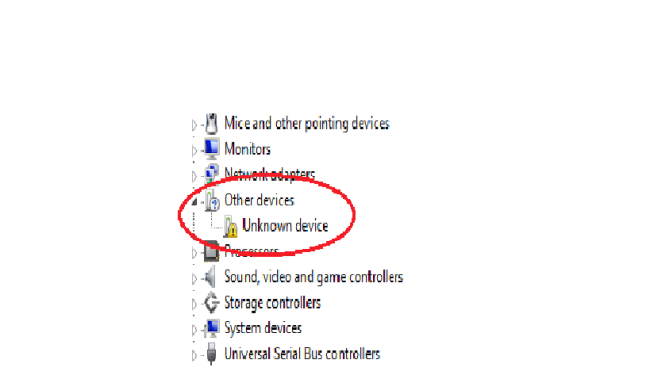
\includegraphics[width=10cm]{figures/5/1174083/Teori/5.png}
				\centering
				\caption{tanda seru.}
			\end{figure}
		\item Klik kanan pada “Unknown device” kemudian pilih Update Driver Software.		
			\begin{figure}[ht]
				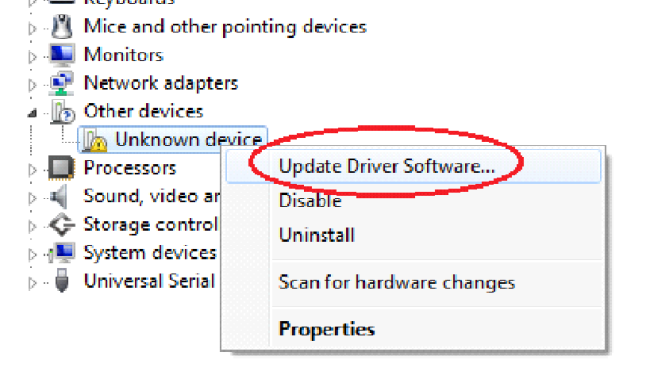
\includegraphics[width=10cm]{figures/5/1174083/Teori/6.png}
				\centering
				\caption{update Driver Software.}
			\end{figure}
		\item Pilih Browse my computer for driver software.
			\begin{figure}[ht]
				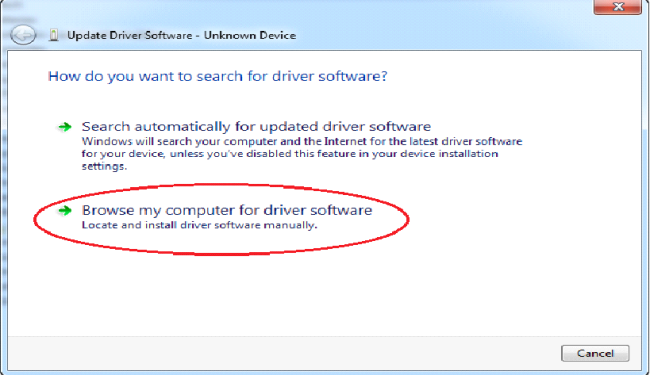
\includegraphics[width=10cm]{figures/5/1174083/Teori/7.png}
				\centering
				\caption{Browse my computer.}
			\end{figure}
		\item Arahkan lokasi folder ke folder \verb|..\arduino-1.0.5\drivers.| Pastikan check-box lalu centang include subfolders. Klik Next untuk melanjutkan instalasi driver.
			\begin{figure}[ht]
				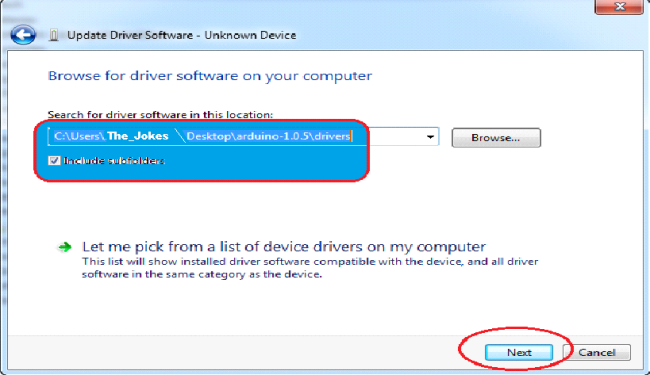
\includegraphics[width=10cm]{figures/5/1174083/Teori/8.png}
				\centering
				\caption{mengarahkan lokasi ke folder.}
			\end{figure}
		\item Kemudian lanjutkan dengan mengklik Install pada tampilan Windows Security.
			\begin{figure}[ht]
				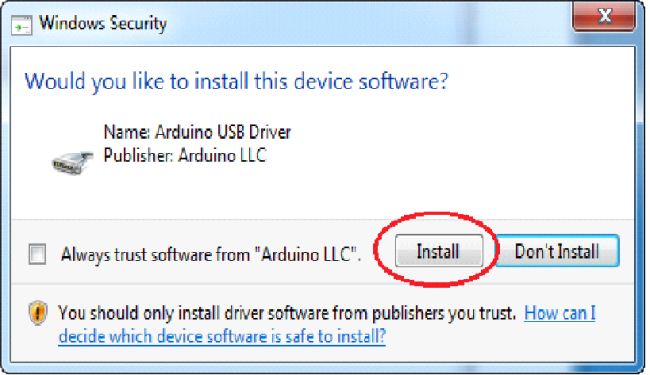
\includegraphics[width=10cm]{figures/5/1174083/Teori/9.png}
				\centering
				\caption{Klik Install.}
			\end{figure}
		\item Jika instalasi driver berhasil maka akan muncul Windows has successfully updated your driver software.
			\begin{figure}[ht]
				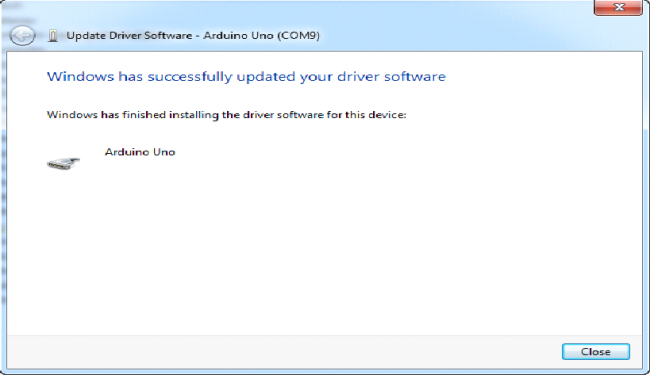
\includegraphics[width=10cm]{figures/5/1174083/Teori/10.png}
				\centering
				\caption{Successfully}
			\end{figure}
		\item Perhatikan dan ingat nama COM Arduino Uno, karena nama COM ini yang akan digunakan untuk meng-upload program nantinya.
			\begin{figure}[ht]
				\includegraphics[width=10cm]{figures/5/1174083/Teori/11.png}
				\centering
				\caption{Selesai.}
			\end{figure}
	\end{itemize}
	
\subsection{Soal 3}
Jelaskan bagaimana cara membaca baudrate dan port dari komputer yang sudah
terinstall driver

Untuk melihat atau membaca baudrate dan port kita hanya perlu menginstall Arduino IDE, setelah itu buka menu serial monitor yang berada di tab tools. Dari sana akan terlihat baik baudrate dan port yang sedang digunakan oleh arduino anda.

\subsection{Soal 4}
Jelaskan sejarah library pyserial

PySerial merupakan sebuah library yang digunakan untuk komunikasi ke port serial terutama untuk mikrokontroller. PySerial pertama kali diluncurkan pada tahun 2002 yang makin berkembang dalam setiap versinya hingga tahun 2017 lalu.

\subsection{Soal 5}
Jelaskan fungsi-fungsi apa saja yang dipakai dari library pyserial

Fungsi-fungsi yang dipakai dari library PySerial, yaitu:
\begin{enumerate}
	\item Serial - fungsi ini untuk membuka port serial.
	\item read(size) - fungsi ini untuk membaca jumlah byte dari port serial.
	\item write(data) - fungsi ini menulis data lewat port serial.
	\item readline() - fungsi ini membaca sebuah string dari port serial.
	\item close() - fungsi ini untuk menutup port serial.
\end{enumerate}

\subsection{Soal 6}
Jelaskan kenapa butuh perulangan dan tidak butuh perulangan dalam membaca serial

Karena dalam pembacaan serial dalam arduino yang memerlukan membaca data secara berulang-ulang harus dengan perulangan. dan tidak butuh perulangan ketika membaca data hanya dilakukan sekali saja.

\subsection{Soal 7}
Jelaskan bagaimana cara membuat fungsi yang mengunakan pyserial

tata cara untuk membuat pyserial seperti pada kode dibawah

\lstinputlisting[firstline=10, lastline=16]{src/5/1174083/Teori/1174083.py}


\subsection{Cek Plagiat}
\begin{figure}[H]
	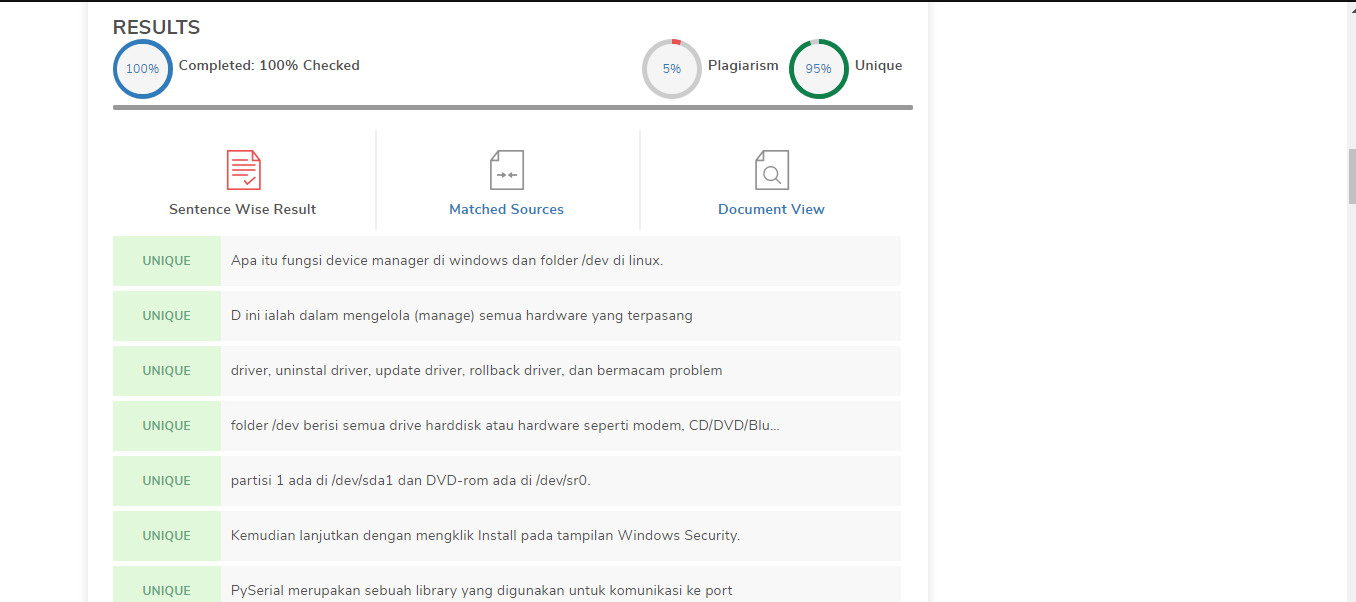
\includegraphics[width=10cm]{figures/5/1174083/Teori/plagiat1.png}
	\centering
	\caption{Hasil cek plagiarism.}
\end{figure}

\subsection{Kode Program}
\begin{figure}[ht]
	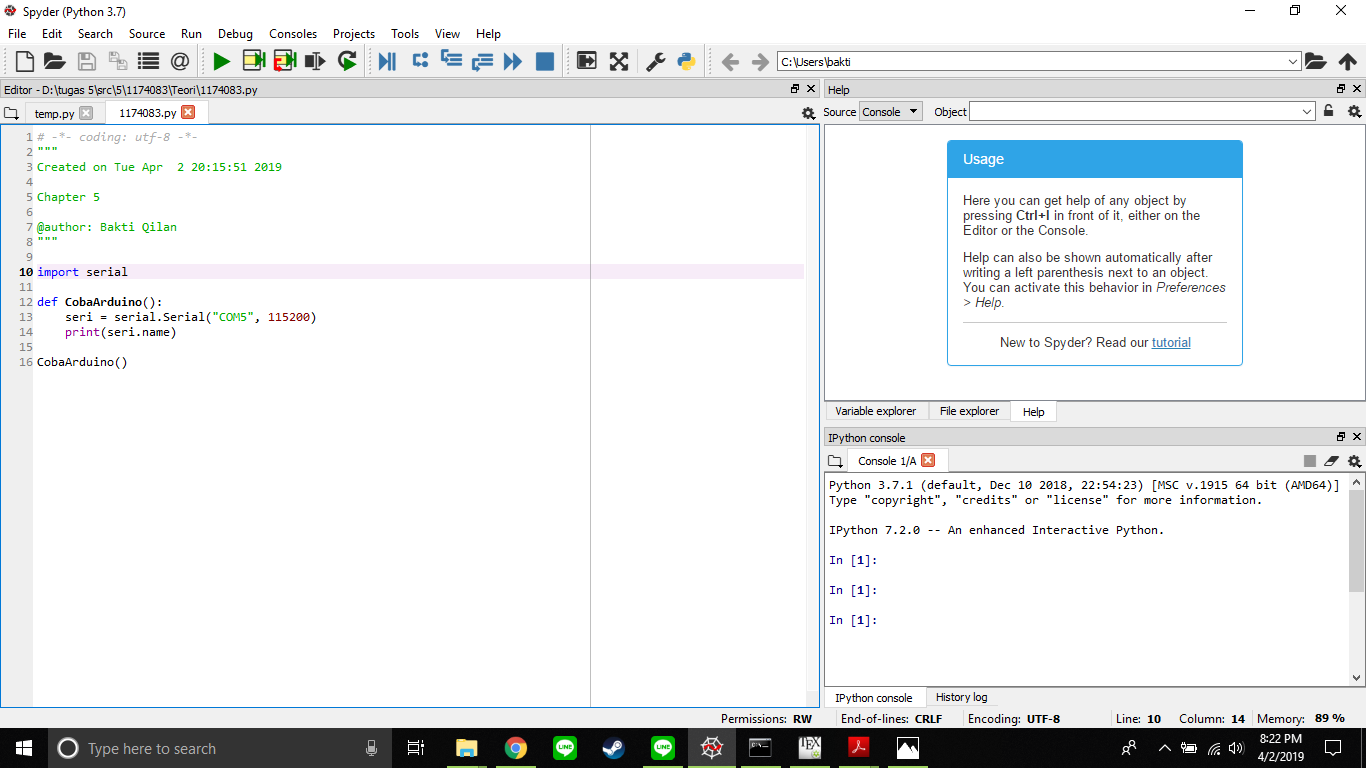
\includegraphics[width=10cm]{figures/5/1174083/Teori/kodefungsi.png}
	\centering
	\caption{Kode program fungsi.}
\end{figure}

%%%%%%%%%%%%%%%%%%%%%%%%%%%%%%%%%%%%%%%%%%%%%%%%%%%%%%%%%%%%%%%%%%%%%%%%%%%%%%%%%%%%%%%%%%%%%%%%%%%%%%%%%
\section{Mochamad Arifqi Ramadhan | 1174074}
\subsection{Soal 1}

\textbf{Fungsi Device manager di Windows  Folder /dev di Linux}
\begin{itemize}
\item Fungsi Device Manager di Windows
	Device Manager akan sangat membantu dalam mengelola (manage) semua hardware yang terpasang (dan terdeteksi) dalam suatu sistem Windows. Hardware seperti harddisk, kartu VGA, sound, keyboard, perangkat USB dll. akan sangat mudah untuk dikonfigurasi dari dalam Device Manager ini. ( mengetahui port arduinno)

\item Fungsi Folder /dev di Linux
/dev berfungsi mengetahui  direktori yang tersimpan konfigurasi device/hardware pada sistem. Contohnya folder /dev artinya file-file tersebut berada.
\end{itemize}
	
\subsection{Soal 2}	
\textbf{Intall Arduino}

Cara instalasi driver arduino :
		\begin{enumerate}
			\item Pertama download software arduino, extract bila file zip/rar
			\item hubungkan Port USB Arduino UNO ke Port USB PC
			\item lalu windows akan memunculkan pop up yang memberitahu bahwa ingin menginstall dirver, tapi nanti tidak akan menemukan drivernya
			\item buka Device Manager, setelah Device Manager terbuka, silahkan cari “Unknown Device” yang berada di Other Device.
			\item klik kanan pada unknown device tersebut lalu pilih update driver software
			\item pilih browse my computer for driver software lalu masukkan directory dimana anda menyimpan driver arduino yang telah anda download tadi
			\item setelah itu klik install dan tunggu hingga proses selesai
			\item arduino pun sudah terbaca di pc anda 
		\end{enumerate}


\subsection{Soal 3}

\textbf{Membaca baudrate dan port di komputer}
Untuk membaca baudrate dan port di komputer pertama hbungkan arduino dengan komputer
1. bisa dengan cara membuka Device manager
2. lalu pilih ports (COM  dan LPT)
3. pilih COM yang terhubung
4. Pilih port setting dan lihat di Bit per second untuk baudrate

Sedangkan untuk port
lakukan proses 1 dan 2 seperti diatas
Dan port dari arduino telah terbaca oleh PC
	
\subsection{Soal 4}

\textbf{Sejarah library PySerial}

	PySerial adalah library yang menyediakan dukungan untuk koneksi serial ("RS-232") melalui berbagai perangkat yang berbeda: port serial gaya lama, dongle Bluetooth, port infra merah, dan sebagainya. Ini juga mendukung port serial jarak jauh melalui RFC 2217 (sejak V2.5). dan PySerial pertama kali diluncurkan pada tahun 2002 yang makin berkembang dalam setiap versinya hingga tahun 2017 lalu.

\subsection{Soal 5}

\textbf{Fungsi-Fungsi di library PySerial}
\begin{itemize}
\item print(ser.name)         - meriksa port yang benar-benar digunakan
\item ser.write(b'hello')     	- menulis tipe data string
\item ser.readline()  	- untuk membaca string dari port serial
\item  ser.read()         	 - membaca satu port
\item ser.close()         	- menutup port
\end{itemize}

\subsection{Soal 6}

\textbf{Perulangan dan Tidak Perulangan}
	Perulangan digunakan untuk melakukan scanning/pengambilan data secara terus menerus(continue) artinya pengeksekusiannya terus berjalan auto selama ada scanning/pengambilan data. Sedangkan Tidak Pengulangan digunakan untuk menscanning/pengambilan data secara real time atau pengambilan datanya hanya sekali saja.


\subsection{Soal 7}

\textbf{Membuat fungsi dengan PySerial}


 Import Serial

Ser = serial.Serial (port, baudrate) membuka serial port
Ketengan : Ser adalah objek Serial, serial adalah kelas, Serial adalah method

contoh fungsi : data = Ser.readline() artinya membaca data


\subsection{Bukti Screenshoot}

\begin{figure}[H]
	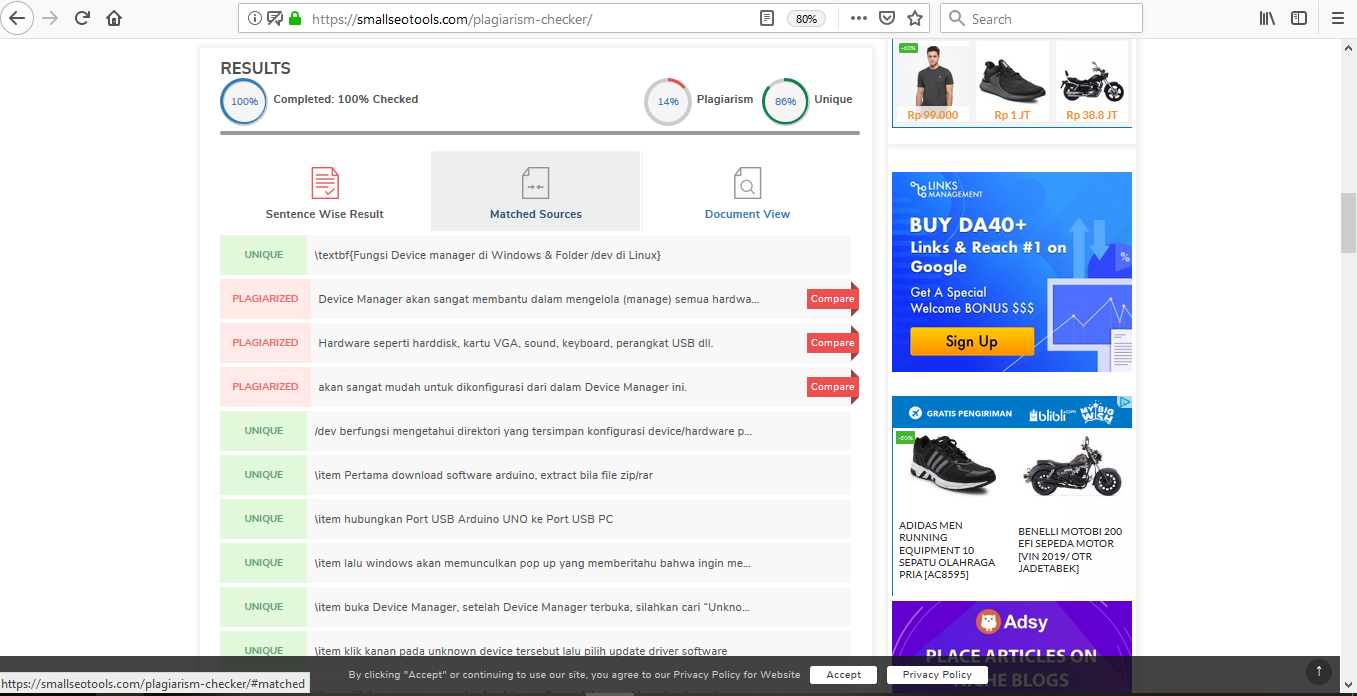
\includegraphics[width=10cm]{figures/5/1174074/Teori/plagiarisme2.png}
	\centering	
	\caption{Cek Plagiat}
\end{figure}
%%%%%%%%%%%%%%%%%%%%%%%%%%%%%%%%%%%%%%%%%%%%%%%%%%%%%%%%%%%%%%%%%%%%%%%%%%%%%%%%%%%%%%%%%%%%%%%%%%%%%%%%%%%%%%%%%%%%


\section{Dini Permata Putri}
\begin{enumerate}

\item Apa itu fungsi device manager di windows dan folder /dev di linux.\\
jawab : \\
Device Manager dalam komputer Windows, adalah perluasan dari Microsoft Management Console. Device Manager menampilkan seluruh hardware yang bisa di-inisialisasi (dikenali) oleh Windows. Tampilannya sudah ter-organisir (dikelompokkan) sedemikian rupa sehingga akan memudahkan pengelolaan setiap hardware yang ada.\\

Fungsi Device Manager Windows\\
Device Manager akan sangat membantu dalam mengelola (manage) semua hardware yang terpasang (dan terdeteksi) dalam suatu sistem Windows. Hardware seperti harddisk, kartu VGA, sound, keyboard, perangkat USB dll. akan sangat mudah untuk dikonfigurasi dari dalam Device Manager ini.\\
folder /dev di linux
Directory ini berisi file device, baik device blok maupun device karakter. di dalamnya minimal harus ada file biner MAKEDEV untuk membuat device ini secara manual.\\

\item Jelaskan langkah-langkah instalasi driver dari arduino\\
jawab :\\
- setalah anda berhasil mengunduh file installer (sekitar 80 Mb), double click-lah file tersebut untuk segera memulai proses instalasi\\
- setelah file installer dijalankan, akan muncul jendela 'Licanse Agreement'. Klik aja tombol 'I Agree'\\
- berikutnya anda akan diminta memasukan folder instalasi Arduino. Biarkan default di C:/Program Files/Arduino. atau kalau mau diganti juga bisa\\
- setelah itu akan muncul jendela 'Setup Installation Options'. Sebaiknya dicentang semua opsinya\\
- selanjutnya proses instalasi dimulai\\
- ditengah proses instalasi, jika komputer anda belum terinstal driver USB, maka akan muncul jendela 'Security Warning' sbb. click tombol instal.\\
- tunggu sampai proses instalasi 'Complated'\\
- pada tahap ini software IDE Arduino sudah terinstal. coba cek di Start Menu Windows anda atau di desktop seharusnya ada ikon Arduino. jika sudah menemukannya, jalankan aplikasi tersebut. dan muncul splash screen\\
- beberapa detik kemudian, jendela IDE Arduino akan muncul\\

\item Jelaskan bagaimana cara membaca baudrate dan port dari komputer yag sudah terinstall driver\\
jawab : \\
untuk membaca baudrate menggunakan Arduino IDE, sedangkan membaca port menggunakan device manager\\

\item Jelaskan sejarah library pyserial\\
jawab :\\
Pyserial adalah library/modul Python siap-pakai dan gratis yang dibuat untuk memudahkan kita dalam membuat program komunikasi data serial RS232 dalam bahasa Python.\\

Jika modul USB-2REL dapat kita kontrol dengan mudah menggunakan Python dan PyUSB (lihat pembahasannya di sini dan di sini), maka modul SER-2REL juga dapat kita kontrol dengan mudah menggunakan Python dengan bantuan modul PySerial.\\

\item jelaskan fungsi-fungsi apa saja yang dipakai dari library pyserial\\
jawab :\\
- SER2REL = serial.Serial(“COM1”, 2400)\\

Jika binding berhasil maka port serial COM1 akan di-open dan siap digunakan. Untuk mengetes apakah COM1 sudah open dan siap digunakan, kita gunakan fungsi isOpen sebagai berikut:\\

- SER2REL.isOpen()\\

Fungsi ini menghasilkan nilai True jika COM1 sudah open dan nilai False jika sebaliknya. Pada eksperimen kita, SER2REL.isOpen() menghasilkan nilai True yang berarti kita sudah dapat mengirim dan menerima data ke dan dari port serial COM1.\\

\item Jelaskan kenapa butuh perulangan dalam tidak butuh perulangan dalam membaca serial\\
jawab :\\
Perulangan atau dalam istilah lain disebut dengan loop. Perulangan digunakan ketika kamu harus menyelesaikan sebuah task dengan jumlah yang besar dengan menggunakan pola yang sama. Syaratnya tentu saja, kamu harus mengetahui bagaimana pola atau alur dari task tersebut. \\

Di dalam Python, ada dua jenis perulangan yang lazim digunakan, yaitu:\\

- For\\
Adalah suatu bentuk perulangan yang mengerjakan ”bagian pernyatan yang sama” secara berulang kali berdasarkan syarat/kondisi yang ditentukan. Cara kerja ini digunakan untuk menyelesaikan task dengan cara yang sama dan dengan hasil yang berbeda.\\

- While\\
Digunakan  untuk melakukan task perulangan selama kondisi nya bernilai benar. Logika pengecakan adalah sama dengan statement IF untuk menentukan benar atau salah. Berikut ini adalah struktur dari while\\

\item Jelaskan bagaimana cara meembuat fungsi yang menggunakan pyserial\\
jawab :\\
membuat fungsi menggunakan pyserial, dibuat dengan kata kunci def kemudian diikuti dengan nama fungsinya.\\
contoh :\\
def nama\_fungsi():\\
	print "Hello ini Fungsi"\\

setelah kita buat, kita bisa mmanggilnya seperti ini:\\
nama\_fungsi()\\
sebagai contoh, coba tulis kode program berikut:\\
sama seperti blok kode yang lain, kita juga harus memberikan identasi (tab atau spasi 2x) untuk menuliskan isi fungsi.\\

\# membuat fungsi\\
def salam():\\
	print "Hello, Selamat Pagi"\\
\#\# pemanggilan fungsi\\
salam()\\
hasilnya : \\
Hello, Selamat Pagi\\

\end{enumerate}
%%%%%%%%%%%%%%%%%%%%%%%%%%%%%%%%%%%%%%%%%%%%%%%%%%%%%%%%%%%%%%%%%%%%%%%%%%%%%%%%%%%%%%%%%%%%%%%%%%%%%%%%%%%%%%%%%%%%%%%%%%%%%%%%%%%%%%%%%%%%%%%%%%%%%%%%%%%%%%%%%%%%%%%%
\section{Arrizal Furqona Gifary}
\subsection{Teori}
\subsubsection{Apa itu fungsi device manager di windows dan folder /dev di linux}
Fungsi device manager dan folder /dev itu berfungsi untuk mengetahui device apa saja yang telah terinstal di leptop anda serta mengetahui port yang digunakan oleh device tersebut.

\subsubsection{Jelaskan langkah-langkah instalasi driver dari arduino}
\begin{enumerate}
    \item Cara Auto
    \begin{itemize}
        \item Pertama Hubungkan sistem minimum Arduino Uno ke komputer dengan kabel USB type B(kabel Printer)
        \begin{figure}[H]	
            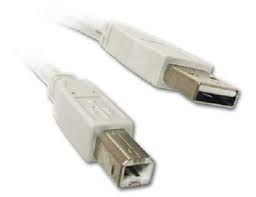
\includegraphics[width=5cm]{figures/5/1174070/teori/1.jpg}
            \centering
            \caption{Membuat file csv}
        \end{figure}

        \item Lalu pada bagian kanan didesktop PC anda, akan muncul popup “Installing device driver software” seperti pada gambar dibawah ini.
        \begin{figure}[H]	
            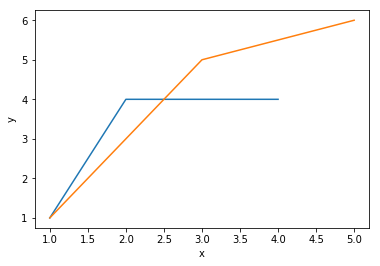
\includegraphics[width=5cm]{figures/5/1174070/teori/2.png}
            \centering
            \caption{Membuat file csv}
        \end{figure}

        \item Tunggu hingga selesai.
        \item Jika sudah selesai anda bisa mengecheck di device manager.
        \begin{figure}[H]	
            \includegraphics[width=5cm]{figures/5/1174070/teori/11.png}
            \centering
            \caption{Membuat file csv}
        \end{figure}
    \end{itemize}

    \item Cara Manual

    \begin{itemize}
        \item Penginstalan secara manual akan dilakukan jika penginstalan secara auto gagal dilakukan.
        \item Buka Device Manager, caranya pada bagian Search Program and Files lalu ketikkan “device manager”, perhatikan gambar dibawah ini. Pada bagian Control Panel akan muncul Device Manager, klik untuk menjalankan.
            \begin{figure}[H]	
                \includegraphics[width=5cm]{figures/5/1174070/teori/4.png}
                \centering
                \caption{Membuat file csv}
            \end{figure}

        \item Cari Unknown device pada bagian Other device, biasanya terdapat tanda seru berwarna kuning, itu disebabkan karena penginstallan tidak berjalan dengan sempurna.
        \begin{figure}[H]	
            \includegraphics[width=5cm]{figures/5/1174070/teori/5.png}
            \centering
            \caption{Membuat file csv}
        \end{figure}

        \item Klik kanan pada “Unknown device” kemudian pilih Update Driver Software.
        \begin{figure}[H]	
            \includegraphics[width=5cm]{figures/5/1174070/teori/6.png}
            \centering
            \caption{Membuat file csv}
        \end{figure}

        \item Pilih Browse my computer for driver software.
        \begin{figure}[H]	
            \includegraphics[width=5cm]{figures/5/1174070/teori/7.png}
            \centering
            \caption{Membuat file csv}
        \end{figure}

        \item Arahkan lokasi folder ke folder ..arduino-1.0.5 drivers. Pastikan check-box lalu centang include subfolders. Klik Next untuk melanjutkan instalasi driver.
        \begin{figure}[H]	
            \includegraphics[width=5cm]{figures/5/1174070/teori/8.png}
            \centering
            \caption{Membuat file csv}
        \end{figure}

        \item Kemudian lanjutkan dengan mengklik Install pada tampilan Windows Security.
        \begin{figure}[H]	
            \includegraphics[width=5cm]{figures/5/1174070/teori/9.png}
            \centering
            \caption{Membuat file csv}
        \end{figure}

        \item Jika instalasi driver berhasil maka akan muncul Windows has successfully updated your driver software.
        \begin{figure}[H]	
            \includegraphics[width=5cm]{figures/5/1174070/teori/10.png}
            \centering
            \caption{Membuat file csv}
        \end{figure}

        \item Perhatikan dan ingat nama COM Arduino Uno, karena nama COM ini yang akan digunakan untuk meng-upload program nantinya.
        \begin{figure}[H]	
            \includegraphics[width=5cm]{figures/5/1174070/teori/11.png}
            \centering
            \caption{Membuat file csv}
        \end{figure}
        \end{itemize}
\end{enumerate}
\subsubsection{Jelaskan bagaimana cara membaca baudrate dan port dari komputer yang sudah terinstall driver}
Untuk baudrate itu bisa dicek melalui arduino IDE, kemudian untuk mengecheck port bisa dilakukan dengan device manager

\subsubsection{Jelaskan sejarah library pyserial}
Modul ini merangkum akses untuk port serial. Ini menyediakan backends untuk Python yang berjalan di Windows, Linux, BSD (mungkin sistem yang mendukung POSIX), Jython dan IronPython (.NET dan Mono). Modul bernama "serial" secara otomatis memilih backend yang sesuai. Antarmuka berbasis kelas yang sama pada semua platform yang didukung.
Akses ke pengaturan port melalui properti Python.
Dukungan untuk berbagai ukuran byte, bit stop, paritas dan kontrol aliran dengan RTS / CTS dan / atau Xon / Xoff.
Bekerja dengan atau tanpa menerima batas waktu.
File seperti API dengan "read" dan "write" ("readline" dll. Juga didukung).
File-file dalam paket ini adalah 100 persen Python murni.
Port diatur untuk transmisi biner. Tidak ada stripping byte NULL, terjemahan CR-LF dll. (Yang berkali-kali diaktifkan untuk POSIX.) Ini membuat modul ini bermanfaat secara universal.
Kompatibel dengan pustaka io (Python 2.6+)

\subsubsection{Jelaskan fungsi-fungsi apa saja yang dipakai dari library pyserial}


Serial – fungsi ini untuk membuka port serial
Write(data) – untuk menulis data lewat port serial
Readline() – untuk membaca string dari port serial
Read(size) – untuk membaca jumlah byte dari port serial
Close() – ini untuk menutup port serial 

\subsubsection{Jelaskan kenapa butuh perulangan dan tidak butuh perulangan dalam membaca serial}


Perualangan dalam bahasa pemrograman berfungsi menyuruh komputer melakukan sesuatu secara berulang-ulang. Terdapat dua jenis perualangan dalam bahasa pemrograman python, yaitu perulangan dengan for dan while.
Perulangan for disebut counted loop (perulangan yang terhitung), sementara perulangan while disebut uncounted loop (perulangan yang tak terhitung). Perbedaannya adalah perulangan for biasanya digunakan untuk mengulangi kode yang sudah diketahui banyak perulangannya. Sementara while untuk perulangan yang memiliki syarat dan tidak tentu berapa banyak perulangannya.
Perulangan diperlukan agar dapat membaca data secara berulang kali sehingga data yang muncul lebih dari satu.  Sedangkan apabila tidak memakai perulangan maka data akan terbaca satu kali saja.

\subsubsection{Jelaskan bagaimana cara membuat fungsi yang mengunakan pyserial}


Berikut merupakan contoh penggunaan fungsi yang menggunakan pyserial
\lstinputlisting[firstline=8, lastline=15]{src/5/1174070/Teori/1174070.py}

\subsubsection{Scan Plagiarisme}
\begin{figure}[H]	
    \includegraphics[width=5cm]{figures/5/1174070/Teori/nopla.png}
    \centering
    \caption{Membuat file csv}
\end{figure}

\subsection{Praktek}
\subsubsection{Buatlah fungsi (file terpisah/library dengan nama NPM realtime.py) untuk mendapatkan data langsung dari arduino}
\lstinputlisting[firstline=8, lastline=14]{src/5/1174070/praktek/1174070_realtime.py}

\subsubsection{Buatlah fungsi (file terpisah/library dengan nama NPM save.py) untuk mendapatkan data langsung dari arduino dengan looping}
\lstinputlisting[firstline=8, lastline=15]{src/5/1174070/praktek/1174070_save.py}

\subsubsection{Buatlah fungsi (file terpisah/library dengan nama NPM realtime.py) untuk mendapatkan data dari arduino dan langsung ditulis kedalam file csv}
\lstinputlisting[firstline=16, lastline=29]{src/5/1174070/praktek/1174070_realtime.py}

\subsubsection{Buatlah fungsi (file terpisah/library dengan nama NPM csv.py) untuk membaca file csv hasil arduino dan mengembalikan ke fungsi}
\lstinputlisting[firstline=8, lastline=16]{src/5/1174070/praktek/1174070_csv.py}

\subsubsection{Penanganan Error}
Untuk kali ini saya menemukan Type Error, yaitu error yang menampilkan jika type data na berbeda berusaha disatukan.
\lstinputlisting[firstline=8, lastline=17]{src/5/1174070/praktek/1174070.py}

%%%%%%%%%%%%%%%%%%%%%%%%%%%%%%%%%%%%%%%%%%%%%%%%%%%%%%%%%%%%%%%%%%%%%%%%%%%%%%%%%%%%%%%%%%%%%%%%%%%%%%%%%%%%%%%%%%%%%%%%%

\section{Muhammad Reza Syachrani / 1174084}
\subsection{Pemahaman Teori}
\begin{enumerate}
    \item fungsi device manager di windows adalah membantu dalam mengelola hardware yang terpasang dalam suatu sistem windows. Sedangkan folder /dev pada linux merupakan direktori yang berfungsi untuk menyimpan konfigurasi device atau hardware dari sistem
    \item langkah-langkah instalasi driver Arduino :
    \begin{enumerate}
        \item Hubungkan sistem Arduino Uno ke computer dengan kabel USB type B
        \item lalu akan muncul popup “Installing device driver software” pada bagian kanan dideskop PC.
        \item Namun, sistem operasi windows tidak menyediakan driver untuk Arduino Uno, sehingga proses instalasinya dilakukan secara manual. Dengan cara membuka Device Manager, pada bagian Search Program and Files kita ketikkan device manager lalu klik
        \item Kemudian cari Other device, kemudian klik dan pilih Unkonown device biasanya bertanda seru berwarna kuning, karena penginstalan tidak berjalan sempurna.
        \item Lalu klik kanan pada “Unknown device” dan pilih Update Driver Software
        \item Pilih Browser my computer for driver software
        \item Lalu arahkan lokasi folder ke \ arduino-1.0.5\ driver. Dan pastikan check-box include subfolder dicentang, kemudian klik next.
        \item Dan lanjut mengklik Install pada tampilan Windows Security
        \item Terakhir akan muncul Windows has successfully update your driver software jika instalasi driver berhasil
        \item Dan ingat nama COM Arduino Uno, karena nama COM yang digunakan untuk meng-upload program nantinya.
    \end{enumerate}
    \item Cara membaca baudrate bisa dilihat menggunakan Arduino Ide dengan cara mengklik icon serial monitor , sedangkan port dapat  dilihat pada device manager
    \item pyserial merupakan sebuah serial module/library yang merangkum akses untuk port serial. Ini menyediakan backends untuk Python yang berjalan di Windows, Linux, BSD. Modul bernama "serial" secara otomatis memilih backend yang sesuai. Pyserial pertama kali diluncurkan pada tahun 2002.
    \item Fungsi-fungsi pada library Pyserial :
    \begin{enumerate}
        \item Serial(), berfungsi untuk membuka port serial
        \item write(), Berfungsi untuk mengirimkan data string ke port serial
        \item readline(), Berfungsi untuk membaca sebuah string dari port serial. 
        \item read(size), Berfungsi untuk membaca data dari port serial
        \item close(), Berfungsi untuk menutup port serial
    \end{enumerate}
    \item Perulangan dibutuhkan saat membaca serial, karena agar data yang dibaca tidak hanya satu kali saja tetapi berkali kali, sehingga dengan adanya perulangan tersebut kita dapat membaca datanya berulang kali. Sedangkan perulangan tidak dibutuhkan ketika kita hanya membutuhkan datanya hanya satu. 
    \item cara membuat fungsi menggunakan pyserial:
    \begin{enumerate}
        \item pertama mengimport library serial dengan cara "import serial"
        \item kemudian membuat fungsi dengan mendefinisikan nama fungsi dengan cara def namafungsi():
        \item lalu masukan isi fungsi dengan library pyserial, seperti serial(), read(), dll.
        \item setelah itu panggil namafungsi().
    \end{enumerate}
    \item Scan Plagiarisme
    \begin{figure}[ht!]
    \includegraphics[width=5cm]{figures/5/1174084/Teori/c5_1.png}
    \centering
    \caption{plagiarisme}
    \end{figure}

\end{enumerate}

%%%%%%%%%%%%%%%%%%%%%%%%%%%%%%%%%%%%%%%%%%%%%%%%%%%%%%%%%%%%%%%%%%%%%%%%%%%%%
%PRAKTEK
%\chapter{Praktek Komunikasi Perangkat Keras}
%\section{Bakti Qilan Mufid}
\subsection{Soal 1}
Buatlah fungsi (file terpisah/library dengan nama \verb|NPM_realtime.py|) untuk mendapatkan data langsung dari arduino

\lstinputlisting[firstline=9, lastline=16]{src/5/1174083/Praktek/1174083_realtime.py}
\begin{figure}[ht!]
	\includegraphics[width=5cm]{figures/5/1174083/Praktek/1.png}
	\centering
	\caption{Membaca Serial tanpa loop}
\end{figure}

\subsection{Soal 2}
Buatlah fungsi (file terpisah/library dengan nama \verb|NPM_save.py|) untuk mendapatkan data langsung dari arduino dengan looping

\lstinputlisting[firstline=10, lastline=18]{src/5/1174083/Praktek/1174083_save.py}


\subsection{Soal 3}
Buatlah fungsi (file terpisah/library dengan nama \verb|NPM_realtime.py|) untuk mendapatkan data dari arduino dan langsung ditulis kedalam file csv
\lstinputlisting[caption="Kode python",firstline=18, lastline=26]{src/5/1174083/Praktek/1174083_realtime.py}
\lstinputlisting[caption="Data yang telah ditulis ke file csv",firstline=0, lastline=10]{src/5/1174083/Praktek/1174083.csv}



\subsection{Soal 4}
Buatlah fungsi (file terpisah/library dengan nama \verb|NPM_csv.py|) untuk membaca file csv hasil arduino dan mengembalikan ke fungsi

\lstinputlisting[firstline=10, lastline=18]{src/5/1174083/Praktek/1174083_csv.py}

\subsection{Ketrampilan Penanganan Error}
Tuliskan peringatan error yang didapat dari mengerjakan praktek ketiga ini, dan jelaskan cara penanganan error tersebut. dan Buatlah satu fungsi yang menggunakan gunakan try except untuk menanggulangi error tersebut.
\begin{itemize}
\item Syntax Errors

Syntax Errors adalah kesalahan pada penulisan syntax atau kode. Solusinya adalah memperbaiki penulisan syntax atau kode

\item Zero Division Error

ZeroDivisonError adalah exceptions yang terjadi saat eksekusi program menghasilkan perhitungan matematika pembagian dengan angka nol (0). Solusinya adalah tidak membagi suatu yang hasilnya nol.

\item Name Error

NameError adalah exception saat kode melakukan eksekusi terhadap local name atau global name yang tidak terdefinisi atau tidak ada. Solusinya adalah memastikan variabel atau function yang akan dipanggil ada didalam program atau tidak salah mengetikannya.

\item Type Error

TypeError adalah exception saat melakukan eksekusi terhadap suatu operasi atau fungsi dengan type object yang tidak sesuai. Solusinya adalah mengkoversi varibelnya sesuai dengan tipe data sesuai dengan yang akan digunakan.

\end{itemize}
\lstinputlisting[firstline=7, lastline=22]{src/5/1174083/Praktek/1174083_error.py}

%TEORI
\chapter{Tugas 6}
\section{Dini Permata Putri}
\begin{enumerate}


\item 1. Apa itu fungsi library Matplotlib
Matplotlib adalah sebuah library pada python yang digunakan untuk membuat diagram. Library ini biasanya menghasilkan ploting 2D.\\

Ada plot untuk menampilkan data secara 2D atau 3D. sehingga kamu dapat menampilkan data yang telah kamu olah sesuai kebutuhan. Matplotlib pun terintegrasi dengan ipython notebook atau jupyter dimana kamu dapat membuat sebuah buku interaktif yang dapat diberi penjelasan dan kode yang disisipkan begitupun hasil plottingnya.\\

\item 2. Jelaskan langkah-langkah membuat sumbu X dan Y di matplotlib.
A. Klik kanan scatter chart dan klik pilih data dalam menu konteks , lalu pilih "Select Data

B.Dalam kotak dialog sumber data dan sumber keluar , klik untuk menyoroti Y pada kolom. lalu klik tombol ubah pada tombol di legenda entrl.

C. Sekarang kotak dialog di edit pada series keluar , abis itu silahkan tukar Nilai seri X dan Nilai seri Y lalu klik tombol OK untuk menutup kedua kotak dialog.\\

\item 3. Jelaskan bagaimana perbedaan fungsi dan cara pakai untuk berbagai jenis(bar,histogram,scatter.dll) jenis plot di matloptlib
Untuk perbedaan fungsi plot yang digunakan adalah bentuk bentuk grafik yang akan di tampilkan sesuai dengan perintah yang digunakan pada pemogramannya.\\

line
    Perintah yang digunakan untuk membuat grafik line sebagai berikut.
x = [2,4,6,5,42,543,5,3,73,64,42,97,63,76,63,8,73,97,\\
23,45,56,89,45,3,23,2,5,78,23,56,67,78,8,3,78,34,67,\\
23,324,234,43,544,54,33,223,443,444,234,76,432,233,23,\\
232,243,222,221,254,222,276,300,353,354,387,364,309]\\



Bar itu di dalam Penggunaan plot bar koordinat x nya itu yang awal, dan untuk Y nya adalah yang kedua.\\

Histrogram itu di dalam penggunaan plot histogram titik x nya bisa tidak sama dengan titik Y. untuk penggunaannya bisa sebagai berikut.\\

scatter untuk penggunaa plot scatter atau bisa juga d bilang diagram titik.\\

Stack plot untuk penggunaan stack plot ini seperti diagram line, tapi ada fill colornya,jadi antar line itu bisa berdekatan.\\

\item 4. Jelaskan bagaimana cara menggunakan legend dan label serta kaitannya dengan fungsi tersebut.
Contoh source code lengkap disertai dengan link "editor" untuk mencoba (try it) dan melihat hasil (preview) kode.\\

Elemen yang akan ditambahkan ke legenda ditentukan secara otomatis, ketika Anda tidak memberikan argumen tambahan.\\

Garis-garis spesifik dapat dikecualikan dari pemilihan elemen legenda otomatis dengan mendefinisikan label dimulai dengan garis bawah.\\

\item 5. Jelaskan apa fungsi dari subplot di matplotlib dan fungsi dari subplot dari matplotlib untuk bisa membuat lebih dari 1 grafik dalam sebuah program.\\

Misalnya, kita dapat membuat sumbu inset di sudut kanan atas sumbu lain dengan mengatur posisi x dan y ke 0,65 yaitu, mulai dari 65 peren dari lebar dan 65 persen  dari ketinggian gambar dan x dan y meluas ke 0,2 yaitu, ukuran sumbu adalah 20 persen  dari lebar dan 20persen dari tinggi gambar.\\

Simple Grids of Subplots itu kebutuhan yang cukup umum sehingga Matplotlib memiliki beberapa rutinitas kenyamanan yang membuatnya mudah dibuat. Level terendah adalah plt.subplot (), yang membuat subplot tunggal di dalam kisi. Seperti yang Anda lihat, perintah ini membutuhkan tiga argumen bilangan bulat — jumlah baris, jumlah kolom, dan indeks plot yang akan dibuat dalam skema ini, yang berjalan dari kiri atas ke kanan bawah.\\
Contohnya:\\
for i in range(1, 7):
    plt.subplot(2, 3, i)
    plt.text(0.5, 0.5, str((2, 3, i)),
             fontsize=18, ha='center')
             
The Whole Grid in One Go itu  membuat grid besar subplot, terutama jika Anda ingin menyembunyikan label sumbu x dan y pada plot bagian dalam. Untuk tujuan ini, plt.subplots () adalah alat yang lebih mudah digunakan.\\
 
\item 6. Sebutkan semua parameter color yang bisa digunakan(contoh: m,c,r,k,...dkk)
Tipe Warna RGB
    Untuk keterangannya sebagai berikut
    R untuk warna Red atau Merah
    G untuk warna Green atau Hijau
    B untuk warna Blue atau Biru.\\
    
Tipe warna CMYK
    Untuk keterangannya sebagai berikut
    C untuk warna Cyan atau Biru Muda
    M untuk warna Mangenta atau Merah Tua
    Y untuk warna Yellow Atau Kuning
    K untuk warna blacK atau Hitam.\\

\item 7. Jelaskan bagaimana cara kerja dari fungsi hist , sertakan ilustrasi dan gambar sendiri.
Untuk fungsi histogram ini kedua titik koordinat boleh tidak sama. Misalnya x nya ada 10 nilai sedangkan Y nya ada 5 nilai, itu tidak akan jadi masalah karena diagram ini digunakan untuk mendata usia dari rentang tertentu atau kebutuhan lainnya.\\

Ini merupakan contoh dari penggunaan histogram.\\

\item 8. Jelaskan lebih dalam tentang parameter dari fungsi pie diantaranya labels , color , startangle , shadow , explode , autopct.
Jika jumlah x <1, maka nilai x memberikan area fraksional secara langsung dan array tidak akan dinormalisasi.\\

labels : Label digunakan untuk mempermudah pembaca dalam membaca diagram pie.\\

color : warna digunakan untuk membedakan antar data.\\

startangle : Digunakan untuk sudut yang digunakan untuk memulai diagram pie tersebut.\\

shadow :  bayangan digunakan untuk membuat bayangan dari setiap diagram pie yang menonjol.\\

explode : explode digunakan untuk mengeluarkan suatu data agar data tersebut terlihat menonjol.\\

autopct : Digunakan sesuai dengan berapa angka dibelakang koma yang kita inginkan.\\

\end{enumerate}
%%%%%%%%%%%%%%%%%%%%%%%%%%%%%%%%%%%%%%%%%%%%%%%%%%%%%%%%%%%%%%%%%%%%%%
\section{Advent Nopele Olasni Damiahan Sihite / 1174089}
\subsection{Teori}
\subsubsection{Soal No. 1}
\hfill \break
Apa itu fungsi library matplotlib?

\hfill \break
Matplotlib merupakan salah satu library Python 2D yang dapat menghasilkan plot dengan kualitas yang tinggi dalam berbagai format dan dapat digunakan di berbagai platform. Matplotlib berfungsi sebagai pembuat grafik di berbagai platform, seperti Python dan Jupyter. Grafik yang dibuat menggunakan Matplotlib bisa dibuat dalam berbagai bentuk, seperti grafik garis, batang, lingkaran, histogram, dan sebagainya.

\subsubsection{Soal No. 2}
\hfill \break
Jelaskan langkah-langkah membuat sumbu X dan Y di matplotlib!

\begin{enumerate}
	\item Pertama import library Matplotlib.	
	\lstinputlisting[firstline=2, lastline=2]{src/6/1174089/Teori/1174089.py}
	
	\item Buat variabel x yang menampung list untuk sumbu x dan variabel y yang menampung list untuk sumbu y.	
	\lstinputlisting[firstline=4, lastline=5]{src/6/1174089/Teori/1174089.py}
	
	\item Panggil fungsi plot dan isi parameter pertama dengan variabel x dan parameter kedua dengan variabel y.
	\lstinputlisting[firstline=7, lastline=7]{src/6/1174089/Teori/1174089.py}	

	\item Lalu panggil plot tadi dengan memanggil fungsi show.
	\lstinputlisting[firstline=9, lastline=9]{src/6/1174089/Teori/1174089.py}
	
\end{enumerate}
\hfill \break
\textbf{Kode Program}

\lstinputlisting[caption = Kode program membuat diagram menggunakan Matplotlib., firstline=2, lastline=9]{src/6/1174089/Teori/1174089.py}

\hfill \break
\textbf{Hasil Compile}

\begin{figure}[H]
	\includegraphics[width=12cm]{figures/6/1174089/Teori/2.png}
	\centering
	\caption{Hasil compile membuat diagram menggunakan Matplotlib.}
\end{figure}
 
\subsubsection{Soal No. 3}
\hfill \break
Jelaskan bagaimana perbedaan fungsi dan cara pakai untuk berbagai jenis(bar, histogram ,scatter ,line, dll) jenis plot di matplotlib!

\begin{enumerate}
	\item \textbf{Bar Graph}
	
	Perbedaan bar graph dengan jenis plot yang lain adalah bar graph menggunakan bar atau batang-batang untuk membandingkan data di antara berbagai kategori.
	
	\textbf{Kode Program}
	
	\lstinputlisting[caption = Kode program membuat bar graph menggunakan Matplotlib., firstline=2, lastline=9]{src/6/1174089/Teori/1174089.py}
	
	\textbf{Hasil Compile}
	
	\begin{figure}[H]
		\includegraphics[width=12cm]{figures/6/1174089/Teori/bar.png}
		\centering
		\caption{Hasil compile membuat bar graph menggunakan Matplotlib.}
	\end{figure}
	
	\item \textbf{Histogram}
	
	Perbedaan histogram dengan jenis plot yang lain adalah histogram akan membuat plot dimana plot yang dimunculkan merupakan gabungan dari beberapa data yang telah dikelompokkan.
	
	\textbf{Kode Program}
	
	\lstinputlisting[caption = Kode program membuat histogram menggunakan Matplotlib., firstline=29, lastline=36]{src/6/1174089/Teori/1174089.py}
	
	\textbf{Hasil Compile}
	
	\begin{figure}[H]
		\includegraphics[width=12cm]{figures/6/1174089/Teori/histogram.png}
		\centering
		\caption{Hasil compile membuat histogram menggunakan Matplotlib.}
	\end{figure}
	
	\item \textbf{Scatter Plot}
	
	Perbedaan scatter plot dengan jenis plot lain adalah scatter plot menampilkan data sebagai kumpulan titik, masing-masing memiliki nilai satu variabel yang menentukan posisi pada sumbu horizontal dan nilai variabel lain menentukan posisi pada sumbu vertikal.
	
	\textbf{Kode Program}
	
	\lstinputlisting[caption = Kode program membuat scatter plot menggunakan Matplotlib., firstline=40, lastline=53]{src/6/1174089/Teori/1174089.py}
	
	\textbf{Hasil Compile}
	
	\begin{figure}[H]
		\includegraphics[width=12cm]{figures/6/1174089/Teori/scatter.png}
		\centering
		\caption{Hasil compile membuat scatter plot menggunakan Matplotlib.}
	\end{figure}
	
	\item \textbf{Area Plot}
	
	Perbedaan area plot dengan jenis plot lain adalah area plot digunakan untuk melacak perubahan dari waktu ke waktu untuk dua atau lebih kelompok terkait yang membentuk satu kategori secara keseluruhan.
	
	\textbf{Kode Program}
	
	\lstinputlisting[caption = Kode program membuat diagram menggunakan Matplotlib., firstline=57, lastline=76]{src/6/1174089/Teori/1174089.py}
	
	\textbf{Hasil Compile}
	
	\begin{figure}[H]
		\includegraphics[width=12cm]{figures/6/1174089/Teori/area.png}
		\centering
		\caption{Hasil compile membuat diagram menggunakan Matplotlib.}
	\end{figure}
	
	\item \textbf{Pie Plot}
	
	Perbedaan pie plot dengan jenis plot lain adalah pie plot digunakan untuk menunjukkan persentase atau data proporsional di mana setiap potongan pie mewakili kategori.
	
	\textbf{Kode Program}
	
	\lstinputlisting[caption = Kode program membuat Pie Plot menggunakan Matplotlib., firstline=80, lastline=101]{src/6/1174089/Teori/1174089.py}
	
	\textbf{Hasil Compile}
	
	\begin{figure}[H]
		\includegraphics[width=9cm]{figures/6/1174089/Teori/pie.png}
		\centering
		\caption{Hasil compile membuat Pie Plot menggunakan Matplotlib.}
	\end{figure}
	
	\item \textbf{Line Graph}
	
	Perbedaan line graph dengan jenis plot lain adalah line graph menampilkan diagram dalam bentuk garis.
	
	\textbf{Kode Program}
	
	\lstinputlisting[caption = Kode program membuat diagram menggunakan Matplotlib., firstline=105, lastline=113]{src/6/1174089/Teori/1174089.py}
	
	\textbf{Hasil Compile}
	
	\begin{figure}[H]
		\includegraphics[width=12cm]{figures/6/1174089/Teori/line.png}
		\centering
		\caption{Hasil compile membuat diagram menggunakan Matplotlib.}
	\end{figure}
	
\end{enumerate}

\subsubsection{Soal No. 4}
\hfill \break
Jelaskan bagaimana cara menggunakan legend dan label serta kaitannya dengan fungsi tersebut!

\begin{enumerate}
	\item Untuk menggunakan legend definisikan parameter label di tiap fungsi plot. Parameter label digunakan untuk memberikan label pada line sebagai pembeda antar line.
	
	\lstinputlisting[caption = Kode program menggunakan parameter label dengan Matplotlib., firstline=123, lastline=124]{src/6/1174089/Teori/1174089.py}
	
	\item Kemudian panggil fungsi legend.
	
	\lstinputlisting[caption = Kode program memanggil fungsi legend dengan Matplotlib., firstline=128, lastline=128]{src/6/1174089/Teori/1174089.py}
\end{enumerate}

\hfill \break
\textbf{Kode Program}

\lstinputlisting[caption = Kode program membuat diagram menggunakan Matplotlib., firstline=117, lastline=130]{src/6/1174089/Teori/1174089.py}

\hfill \break
\textbf{Hasil Compile}

\begin{figure}[H]
	\includegraphics[width=12cm]{figures/6/1174089/Teori/4.png}
	\centering
	\caption{Hasil compile membuat diagram menggunakan Matplotlib.}
\end{figure}

\subsubsection{Soal No. 5}
\hfill \break
Jelaskan apa fungsi dari subplot di matplotlib, dan bagaimana cara kerja dari fungsi subplot, sertakan ilustrasi dan gambar sendiri dan apa parameternya jika ingin menggambar plot dengan 9 subplot di dalamnya!

\hfill \break
Fungsi subplot adalah untuk membuat beberapa plot di dalam satu gambar.
\hfill \break
Cara kerja subplot, yaitu fungsi subplot memiliki parameter pertama adalah jumlah kolom, parameter kedua adalah jumlah baris, dan parameter ketiga adalah index plot keberapanya.

\hfill \break
\textbf{Kode Program}

\lstinputlisting[caption = Kode program membuat subplot menggunakan Matplotlib., firstline=134, lastline=146]{src/6/1174089/Teori/1174089.py}

\hfill \break
\textbf{Hasil Compile}

\begin{figure}[H]
	\includegraphics[width=12cm]{figures/6/1174089/Teori/subplot.png}
	\centering
	\caption{Hasil compile membuat subplot menggunakan Matplotlib.}
\end{figure}

\subsubsection{Soal No. 6}
\hfill \break
Sebutkan semua parameter color yang bisa digunakan (contoh:  m,c,r,k,...  dkk)!

\begin{itemize}
	\item 'b' (blue)
	\item 'g' (green)
	\item 'r' (red)
	\item 'c' (cyan)
	\item 'm' (magenta)
	\item 'y' (yellow)
	\item 'k' (black)
	\item 'w' (white)
\end{itemize}

\subsubsection{Soal No. 7}
\hfill \break
Jelaskan bagaimana cara kerja dari fungsi hist, sertakan ilustrasi dan gambar sendiri!

\hfill \break
Cara kerja dari fungsi hist yaitu fungsi hist akan menerima parameter yang diberikan, kemudian fungsi hist akan dieksekusi sesuai dengan parameter yang diberikan.

\hfill \break
\textbf{Kode Program}

\lstinputlisting[caption = Kode program membuat diagram menggunakan Matplotlib., firstline=150, lastline=157]{src/6/1174089/Teori/1174089.py}

\hfill \break
\textbf{Hasil Compile}

\begin{figure}[H]
	\includegraphics[width=12cm]{figures/6/1174089/Teori/histogram.png}
	\centering
	\caption{Hasil compile membuat diagram menggunakan Matplotlib.}
\end{figure}

\subsubsection{Soal No. 8}
\hfill \break
 Jelaskan lebih mendalam tentang parameter dari fungsi pie diantaranya labels, colors, startangle, shadow, explode, autopct!
 
 \begin{itemize}
 	\item labels : untuk memberikan label di tiap persentase.
 	\item colors : untuk memberikan warna di tiap persentase.
 	\item startangle : untuk memutar plot sesuai dengan derajat yang ditentukan.
 	\item shadow : untuk memberikan bayangan pada plot.
 	\item explode : untuk memisahkan antar tiap potongan pie pada plot.
 	\item autopct : untuk menentukan jumlah angka dibelakang koma.
 \end{itemize}

\subsection{Praktek}
\subsubsection{Soal No. 1}
\hfill \break
Buatlah librari fungsi (file terpisah/library dengan nama NPMbar.py) untuk plot dengan jumlah subplot adalah NPM mod 3 + 2!

\subsubsection{Soal No. 2}
\hfill \break
Buatlah librari fungsi (file terpisah/library dengan nama NPMscatter.py) untuk plot dengan jumlah subplot NPM mod 3 + 2!

\subsubsection{Soal No. 3}
\hfill \break
Buatlah librari fungsi (file terpisah/library dengan nama NPMpie.py) untuk plot dengan jumlah subplot NPM mod 3 + 2!

\subsubsection{Soal No. 4}
\hfill \break
Buatlah librari fungsi (file terpisah/library dengan nama NPMplot.py) untuk plot dengan jumlah subplot NPM mod 3 + 2


\subsection{Penanganan Error}
Tuliskan  peringatan  error  yang  didapat  dari  mengerjakan  praktek  keenam  ini, dan  jelaskan  cara  penanganan  error  tersebut. dan  Buatlah  satu  fungsi  yang menggunakan try except untuk menanggulangi error tersebut.
%%%%%%%%%%%%%%%%%%%%%%%%%%%%%%%%%%%%%%%%%%%%%%%%%%%%%%%%%%%%%

\bibliographystyle{IEEEtran}
%\def\bibfont{\normalsize}
\bibliography{references}


%%%%%%%%%%%%%%%
%%  The default LaTeX Index
%%  Don't need to add any commands before \begin{document}
\printindex

%%%% Making an index
%%
%% 1. Make index entries, don't leave any spaces so that they
%% will be sorted correctly.
%%
%% \index{term}
%% \index{term!subterm}
%% \index{term!subterm!subsubterm}
%%
%% 2. Run LaTeX several times to produce <filename>.idx
%%
%% 3. On command line, type  makeindx <filename> which
%% will produce <filename>.ind
%%
%% 4. Type \printindex to make the index appear in your book.
%%
%% 5. If you would like to edit <filename>.ind
%% you may do so. See docs.pdf for more information.
%%
%%%%%%%%%%%%%%%%%%%%%%%%%%%%%%

%%%%%%%%%%%%%% Making Multiple Indices %%%%%%%%%%%%%%%%
%% 1.
%% \usepackage{multind}
%% \makeindex{book}
%% \makeindex{authors}
%% \begin{document}
%%
%% 2.
%% % add index terms to your book, ie,
%% \index{book}{A term to go to the topic index}
%% \index{authors}{Put this author in the author index}
%%
%% \index{book}{Cows}
%% \index{book}{Cows!Jersey}
%% \index{book}{Cows!Jersey!Brown}
%%
%% \index{author}{Douglas Adams}
%% \index{author}{Boethius}
%% \index{author}{Mark Twain}
%%
%% 3. On command line type
%% makeindex topic
%% makeindex authors
%%
%% 4.
%% this is a Wiley command to make the indices print:
%% \multiprintindex{book}{Topic index}
%% \multiprintindex{authors}{Author index}

\end{document}

